% Basic settings
\documentclass[a4paper,8pt,landscape]{article}
\usepackage[utf8]{inputenc}
\usepackage[german]{babel}

% Layout settings
\usepackage[top=1.1cm, bottom=1.5cm, left=1cm, right=1cm, headsep=5pt]{geometry}
\usepackage[compact]{titlesec}
\titlespacing{\section}{0pt}{0pt}{0pt}
\titlespacing{\subsection}{0pt}{0pt}{0pt}
\titlespacing{\subsubsection}{0pt}{0pt}{0pt}
\setlength{\parindent}{0em}
\setlength{\parskip}{0.2em}

% Remove space before and after math environments
\setlength{\abovedisplayskip}{0pt}
\setlength{\belowdisplayskip}{0pt}

% Itemize settings
\usepackage{enumitem}
\setlist{topsep=0pt, partopsep=0pt, parsep=0pt, itemsep=2pt, leftmargin=14pt}

% My colors
\usepackage[table,dvipsnames]{xcolor}
\definecolor{babyblue}{HTML}{A1CAF1}
\definecolor{peach}{HTML}{EFC9AF}
\definecolor{crayola}{HTML}{FFEE93}

% Custom section formatting
\newcommand{\sect}[1]{\section*{\colorbox{babyblue}{\makebox[\linewidth][l]{#1}}}}
\newcommand{\ssect}[1]{\subsection*{\colorbox{peach}{\makebox[\linewidth][l]{#1}}}}
\newcommand{\sssect}[1]{\subsubsection*{\colorbox{crayola}{\makebox[\linewidth][l]{#1}}}}

% Two columns
\usepackage{multicol}
\setlength{\multicolsep}{5pt}

% Package to include images/sketches
\usepackage{graphicx}

% Mathematical typesetting & symbols
\usepackage{amsfonts}
\usepackage{amsmath}
\usepackage{amssymb}
\usepackage{amsthm}
\usepackage{bigints}
\usepackage{mathtools}
\usepackage{wasysym}
% Package to place sub- and superscripts on the left side of variables
\usepackage{leftidx}

\usepackage{array}
\newcolumntype{C}{>{{}}c<{{}}}
\setlength{\arraycolsep}{2pt}

% Math helper stuff
\newcommand{\N}{\mathbb{N}}
\newcommand{\Z}{\mathbb{Z}}
\newcommand{\R}{\mathbb{R}}
\newcommand{\Q}{\mathbb{Q}}
\newcommand{\E}{\mathbb{E}}
\newcommand{\F}{\mathbb{F}}
\newcommand{\V}{\mathbb{V}}
\renewcommand{\P}{\mathbb{P}}
\newcommand{\true}{\texttt{true}}
\newcommand{\false}{\texttt{false}}
\newcommand{\bigO}{\mathcal{O}}
\newcommand{\comp}{\;\circ\;}
\newcommand{\diff}[1]{\,\mathrm{d}#1}

% Linear algebra custom commands
\newcommand{\B}{\mathcal{B}} % Basis B
\newcommand{\C}{\mathcal{C}} % Basis C
\renewcommand{\S}{\mathcal{S}} % Standardbasis
\renewcommand{\ker}{\text{Ker}}
\newcommand{\im}{\text{Im}}

% Draw stuff
\usepackage{tikz-cd}
\usepackage{paracol}

% Comment packages
\usepackage{verbatim}
\usepackage{comment}

% Path to graphics
\graphicspath{{images/}}

% Package to highlight text
\usepackage{soul}

% Header
\usepackage{fancyhdr}
\usepackage{adjustbox}
\usepackage{lipsum}
\pagestyle{fancy}
\renewcommand{\headrulewidth}{0.4pt}
\renewcommand{\footrulewidth}{0.4pt}
\lhead{Lineare Algebra}
\rhead{Adrian Martinez}

\begin{document}
    \begin{multicols*}{3}
        \raggedcolumns

        \sect{Matrizen}

\ssect{Definition}

Unter einer $m \times n$ \textbf{Matrix} versteht man ein rechteckiges Zahlenschema von doppelt indizierten Grössen $a_{ij}$ mit $m$ waagerecht angeordneten Zeilen und $n$ senkrecht angeordneten Spalten.

\ssect{Rechnen mit Matrizen}

\sssect{Skalare Multiplikation}

Die \textbf{skalare Multiplikation} der $m \times n$ Matrix $A$ mit dem reellen Skalar $\lambda$ ist definiert durch die elementweise Multiplikation mit der Zahl $\lambda$:
\[\lambda A = \lambda \left(
\begin{array}{ccc}
    a_{11} & \ldots & a_{1n} \\
    \vdots & \ddots & \vdots \\
    a_{m1} & \ldots & a_{mn}
\end{array}
\right) = \left(
\begin{array}{ccc}
    \lambda a_{11} & \ldots & \lambda a_{1n} \\
    \vdots         & \ddots & \vdots         \\
    \lambda a_{m1} & \ldots & \lambda a_{mn}
\end{array}
\right)\]

\textbf{Rechenregeln:}

$\lambda$ und $\mu$ sind reelle Skalare, $A$ und $B$ sind $m \times n$ Matrizen.
Dann gilt:
\begin{itemize}
    \item Assoziativgesetz: $\lambda (\mu A) = \mu (\lambda A) = (\lambda \mu) A$
    \item Distributivgesetz 1: $(\lambda + \mu) A = \lambda A + \mu A$
    \item Distributivgesetz 2: $\lambda (A + B) = \lambda A + \lambda B$
\end{itemize}

Für Matrizen $A_1, \dots, A_p$ derselben Grösse und Skalare $\lambda_1, \dots, \lambda_p$ heisst $\lambda_1 A_1 + \dots + \lambda_p A_p$ die \textbf{Linearkombination} von $A_1, \dots, A_p$ mit Koeffizienten $\lambda_1, \dots, \lambda_p$.

\sssect{Multiplikation von Matrizen}

Gegeben seien die Matrizen $A \in \R^{m \times n}$ und $B \in \R^{n \times p}$.
Die \textbf{Produktmatrix} $C = AB$ ist eine $m \times p$ Matrix:
\[c_{ij} = a_{i1} b_{1j} + \dots + a_{in} b_{nj} = \sum_{k=1}^{n} a_{ik} b_{kj}\]
Mit anderen Worten: $c_{ij}$ ergibt sich aus der $i$-te Zeile der Matrix $A$ mal die $j$-te Spalte der Matrix $B$.

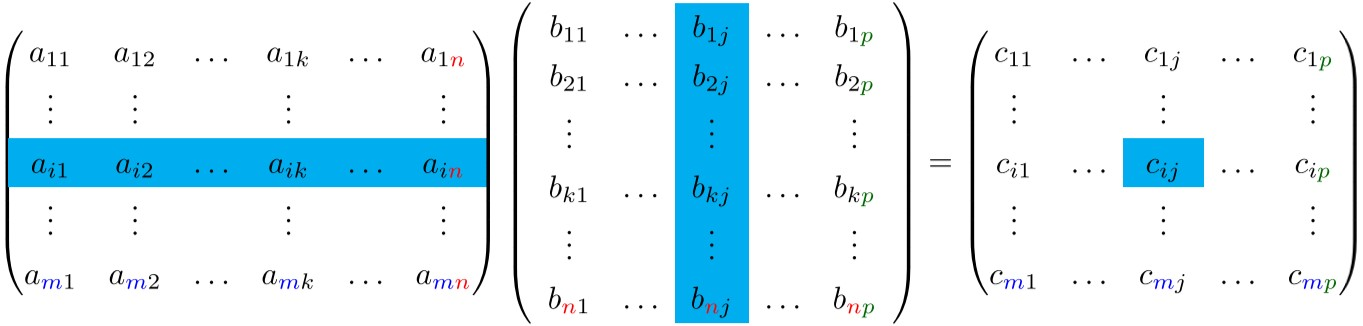
\includegraphics[scale=0.255]{dot-product}

Die Anzahl von Spalten in $A$ muss gleich der Anzahl von Zeilen in $B$ sein!

Das Matrizenprodukt ist generell \textbf{nicht kommutativ}: $AB \neq BA$!

\ssect{Inverse Matrix}

Gibt es zu einer $n \times n$ Matrix $A$ eine Matrix $X$ mit $AX = XA = I_n$, so heisst $X$ die zu $A$ inverse Matrix.
Sie wird durch das Symbol $A^{-1} gekennzeichnet.$

\textbf{Anmerkung:}
\begin{itemize}
    \item Falls eine quadratische Matrix $A$ eine Inverse $A^{-1}$ besitzt, so ist $A^{-1}$ eindeutig bestimmt.
    Die Matrix $A$ heisst in diesem Fall \textbf{invertierbar} (oder \textbf{umkehrbar}).
    Andernfalls heisst sie \textbf{singulär}.
    \item Es gilt: $AA^{-1} = A^{-1}A = I_n$.
    Das heisst, dass $A$ und $A^{-1}$ kommutativ sind.
\end{itemize}

\textbf{Satz:} Das Produkt $AB$ zweier invertierbarer Matrizen ist invertierbar.
Die Inverse zu $AB$ lautet: $(AB)^{-1} = B^{-1} A^{-1}$

\sssect{Berechnung}

Die Matrix $A = \left(
\begin{array}{cc}
    a & b \\ c & d
\end{array} \right) \in \R^{n \times n}$ ist für $\det(A) = ad - bc \neq 0$ invertierbar.
In diesem Fall gilt:
\[A^{-1} = \frac{1}{\det(A)} \left(
\begin{array}{cc}
    d & -b \\ -c & a
\end{array}
\right)\]
Für eine $n \times n$ Matrix $A$ berechnet man $A^{-1}$ wie folgt:
\begin{itemize}
    \item Wir betrachten die erweiterte Koeffizientenmatrix:
    \[(A | I_n) = \left(
    \begin{array}{cccc|cccc}
        a_{11} & a_{12} & \ldots & a_{1n} & 1      & 0      & \ldots & 0      \\
        a_{21} & a_{22} & \ldots & a_{2n} & 0      & 1      & \ldots & 0      \\
        \vdots & \vdots & \ddots & \vdots & \vdots & \vdots & \ddots & \vdots \\
        a_{n1} & a_{n2} & \ldots & a_{nm} & 0      & 0      & \ldots & 1
    \end{array}
    \right)\]
    \item Mit Gauss-Jordan-Verfahren auf reduzierte ZSF bringen.
    \item Ist der \textbf{Rang der Matrix $A$ gleich $n$}, dann lässt sich $A^{-1}$ direkt an der reduzierten ZSF ablesen.

    \[\left(
    \begin{array}{cccc|cccc}
        1      & 0      & \ldots & 0      & x_{11} & x_{12} & \ldots & x_{1n} \\
        0      & 1      & \ldots & 0      & x_{21} & x_{22} & \ldots & x_{2n} \\
        \vdots & \vdots & \ddots & \vdots & \vdots & \vdots & \ddots & \vdots \\
        0      & 0      & \ldots & 1      & x_{n1} & x_{n2} & \ldots & x_{nm}
    \end{array}
    \right) = (I_n | A^{-1})\]
    Ist der \textbf{Rang der Matrix $A$ kleiner als $n$}, dann gibt es keine Inverse.
\end{itemize}

\ssect{Transponierte Matrix}

Sei $A$ eine $m \times n$ Matrix.
Die \textbf{transponierte Matrix} $A^T$ erhält man aus $A$, indem man die $i$-te Spalte von $A$ zur $i$-ten Zeile von $A^T$ macht.
Kurz: $\left[ A^T \right]_{ij} = a_{ij}$

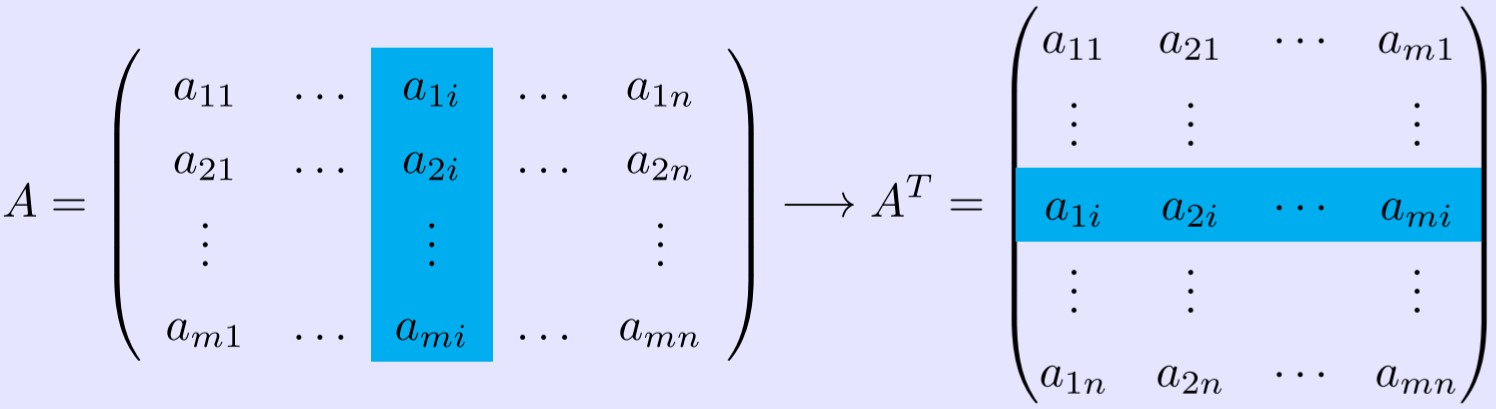
\includegraphics[scale=0.23]{transponierte}

\textbf{Anmerkung:}
\begin{itemize}
    \item Ist $A$ eine $m \times n$ Matrix, so ist ihre Transponierte $A^T$ eine $n \times m$ Matrix.
    \item $(A^T)^T = A$
    \item Durch Transponieren geht ein Zeilenvektor in einen Spaltenvektor über und umgekehrt.
    \item Es gilt für eine symmetrische Matrix $A$ stets: $A^T = A$
\end{itemize}

\textbf{Rechenregeln:}
\begin{enumerate}
    \item $(A + B)^T = A^T + B^T$ für alle $m \times n$ Matrizen $A$ und $B$.
    \item $(\lambda A)^T = \lambda A^T$ $\forall A \in \R^{m \times n}$ und $\forall \lambda \in \R$
    \item $(AB)^T = B^T A^T$ für $A \in \R^{m \times n}$ und $B \in \R^{n \times p}$
    \item $(A^T)^{-1} = (A^{-1})^T$ für eine invertierbare $n \times n$ Matrix $A$
\end{enumerate}

        \sect{LGS}

Eine \textbf{lineare Gleichung in $n$ Variablen} $x_1, \dots, x_n$ hat die Gestalt:
\[a_1 x_1 + \dots + a_n x_n = b\]
wobei $a_1, \dots, a_n$ und $b$ gegebene reelle Konstanten sind.
Die reellen Zahlen $a_i$ mit $i = 1, \dots, n$ nennt man die \textbf{Koeffizienten} der Gleichung und $b \in \R$ ist die \textbf{rechte Seite} der Gleichung.

Ein \textbf{lineares Gleichungssystem} (LGS) besteht aus $m$ linearen Gleichungen mit $n$ Unbekannten $x_1, \dots, x_n$.
Ein solches System hat die folgende Gestalt:
\[
    \setlength\arraycolsep{0pt}
    \left\{
    \begin{array}{*{3}{cC}c}
        a_{11} x_1 & + & \ldots & + & a_{1n} x_n & = & b_1    \\
        \vdots     & + & \vdots & + & \vdots     & = & \vdots \\
        a_{m1} x_1 & + & \ldots & + & a_{mn} x_n & = & b_m
    \end{array}
    \right.
\]

% TODO: Koeffizientenmatrix und Erweiterte Koeffizientenmatrix

\ssect{Elementare Umformungen}

\textbf{Elementare Gleichungsumformungen:}
\begin{itemize}
    \item Vertauschen von den $i$-ten und $j$-ten Gleichungen
    \item Multiplikation der $i$-ten Gleichung mit Skalar $\lambda \neq 0$
    \item Addition eines $\lambda$-fachen der $j$-ten Gleichung zu der $i$-ten Gleichung
\end{itemize}

\textbf{Satz:} Elementare Gleichungsumformungen ändern die Lösungsmenge eines LGS nicht.

\textbf{Elementare Zeilenumformungen:}
\begin{itemize}
    \item Vertauschen von den $i$-ten und $j$-ten Zeilen
    \item Multiplikation der $i$-ten Zeilen mit einem Skalar $\lambda \neq 0$
    \item Addition eines $\lambda$-fachen der $j$-ten Zeile zu der $i$-ten Zeile
\end{itemize}

\ssect{Zeilenstufenform}

Eine Matrix hat \textbf{Zeilenstufenform (ZSF)}, wenn:
\begin{itemize}
    \item Alle Zeilen, die nur Nullen enthalten, stehen in den untersten Zeilen der Matrix.
    \item Wenn eine Zeile nicht nur aus Nullen besteht, so ist die erste von Null verschiedene Zahl eine Eins.
    Sie wird als \textbf{führende Eins} der Zeile bezeichnet.
    \item In zwei aufeinanderfolgenden Zeilen, die nicht verschwindende Elemente besitzen, steht die führende Eins der unteren Zeile rechts von der führenden Eins der oberen Zeile.
\end{itemize}

Eine Matrix in ZSF ist zudem in der \textbf{reduzierten Zeilenstufenform}, falls
\begin{itemize}
    \item eine Spalte, die eine führende Eins enthält, keine weiteren von Null verschiedenen Einträge hat
\end{itemize}

\ssect{Gauss-Jordan-Verfahren}

\begin{enumerate}
    \item Wir bestimmen die am weitesten Links stehende Spalte, die von Null verschiedene Werte enthält.
    \item Ist die oberste Zahl der in Schritt 1 gefundenen Spalte eine Null, dann vertauschen wir die erste Zeile mit einer geeigneten anderen Zeile (1. Zeilenumformung).
    \item Ist $a$ das erste Element der in Schritt 1 gefundene Spalte, dann dividieren wir die erste Zeile durch $a$, um die führende Eins zu erzeugen.
    Man nennt das Element $a$ das Pivotelement (2. Zeilenumformung).
    \item Wir addieren passende Vielfache der ersten Zeile zu den übrigen Zeilen, um unterhalb der führenden Eins Nullen zu erzeugen (3. Zeilenumformung).
    \item Wir wenden die ersten vier Schritte auf den Teil der Matrix an, den wir durch Streichen der ersten Zeile erhalten, und wiederholen dieses Verfahren, bis die erweiterte Koeffizientenmatrix Zeilenstufenform hat.
    \item Mit der letzten nicht verschwindenden Zeile beginnend, addieren wir geeignete Vielfache jeder Zeile zu den darüber liegenden Zeilen, um über den führenden Einsen Nullen zu
    erzeugen (3. Zeilenumformung).
\end{enumerate}

\ssect{Gauss-Verfahren}

\begin{enumerate}
    \item Wir führen die Schritte 1.\ bis 5.\ wie beim Gauss-Jordan-Verfahren durch.
    \item Wir lösen das System in ZSF durch Rückwärtseinsetzen.
\end{enumerate}

\ssect{Lösungsmenge von LGS}

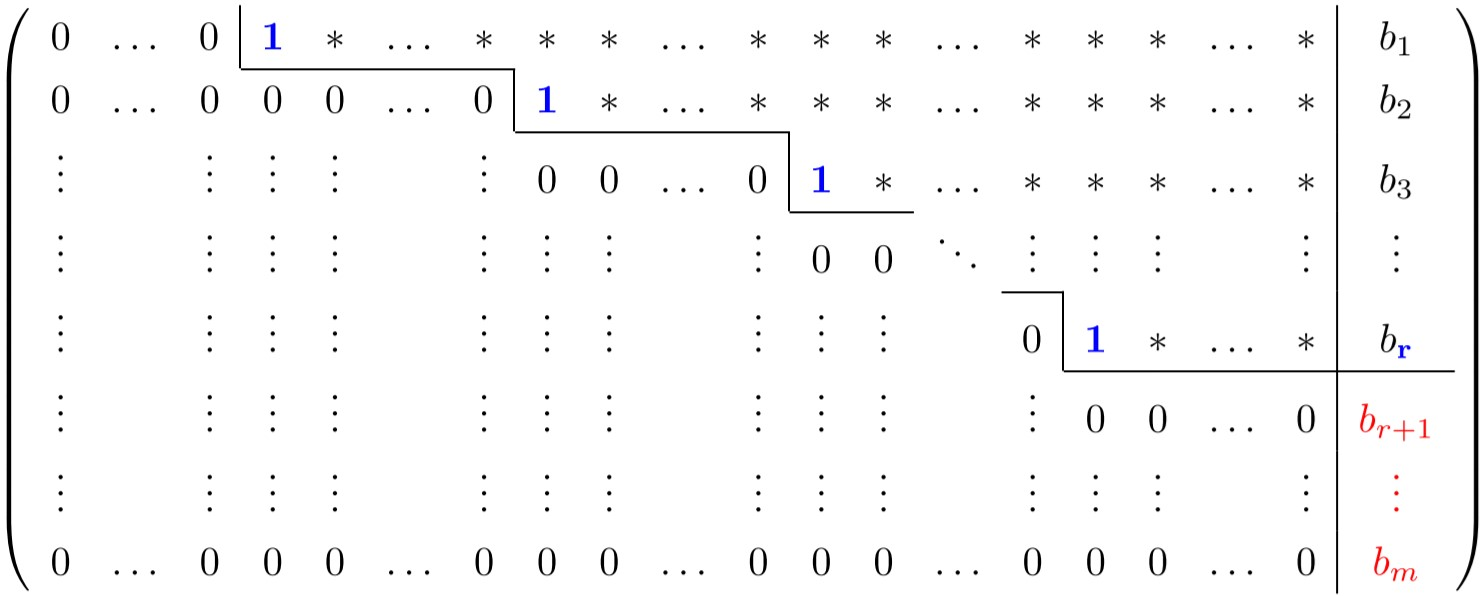
\includegraphics[scale=0.233]{zeilenstufenform}

Sei $r$ die Anzahl der Nicht-Nullzeilen in der ZSF der Koeffizientenmatrix $A$.
Dann heisst $r$ der Rang der Matrix $A$.

\textbf{Anmerkung:}
\begin{itemize}
    \item Es gilt: $r \geq 0$ und $r \leq m$
    \item Die Anzahl der führenden Variablen ist gleich $r$.
    Somit muss auch $r \leq n$ gelten.
    \item Es gibt $n - r$ freie Variablen.
\end{itemize}

Seien $A \vec{x} = \vec{b}$ ein LGS mit $m$ Gleichungen und $n$ Unbekannten, und $r = rg(A)$.\\
Das LGS ist nur \textbf{lösbar}, wenn: $r = rg(A \mid \vec{b})$\\
D.h.\ wenn entweder $r < m$ und $b_k = 0$, $k = r + 1, \dots, m$ oder $r = m$.

Im Falle der Lösbarkeit besitzt das LGS:
\begin{itemize}
    \item Für $r = n$: \textbf{Genau eine Lösung}
    \item Für $r < n$: \textbf{Unendlich viele Lösungen}, wobei die Anzahl der freien Variablen gleich $n - r$ ist.
\end{itemize}

\columnbreak

% TODO: Berechnung der Inverse Matrix

        \sect{Determinante}

\ssect{Definition}

Eine \textbf{$n$-reihige Determinante} ist eine reelle Zahl, die aus den Elementen einer reellen $n \times n$ Matrix nach bestimmten Vorschriften berechnet wird.

Für 2-reihige Determinanten: $\det(A) = \left|
\begin{array}{cc}
    a & b \\
    c & d \\
\end{array}
\right| = ad - cb$

Für 3-reihige Determinante: Regel von Sarrus

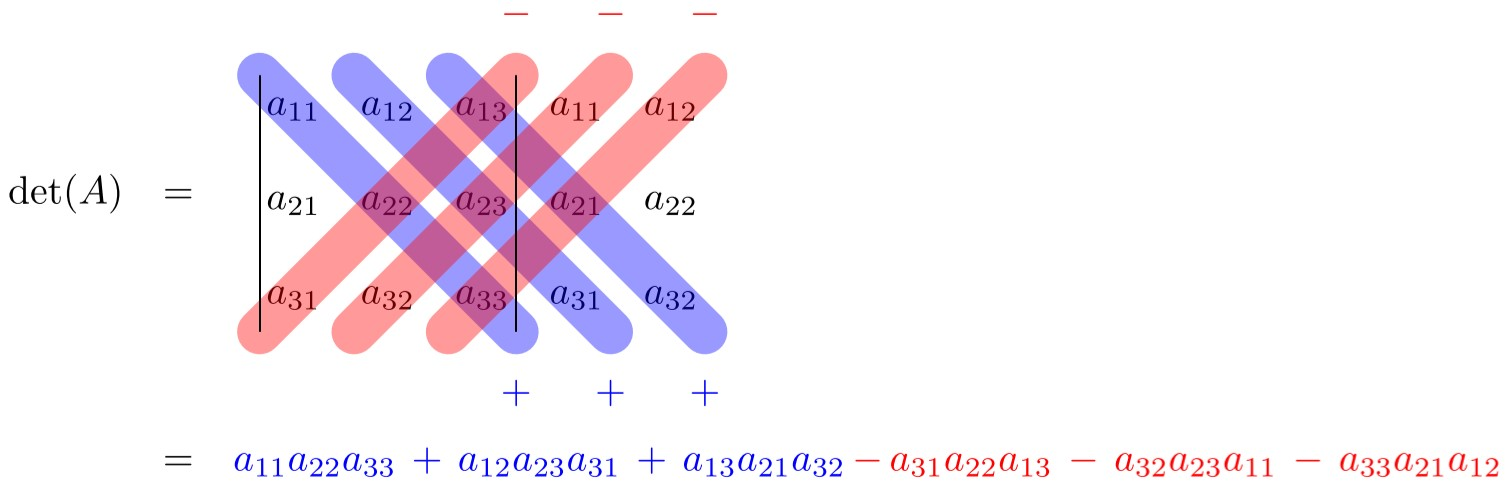
\includegraphics[scale=0.23]{regel-von-sarrus}

\ssect{Eigenschaften}

\textbf{Eigenschaft 1:} Die Matrix $A$ und ihre Transponierte $A^T$ besitzen dieselbe Determinante: $\det(A^T) = \det(A)$

\textbf{Eigenschaft 2:} Beim Vertauschen zweier Zeilen (oder Spalten) ändert eine Determinante ihr Vorzeichen.

\textbf{Eigenschaft 3:} Sei $A$ eine $n \times n$ Matrix.
Sei $\lambda$ eine reelle Zahl.
Dann gilt: $\det(\lambda A) = \lambda^n \det(A)$

\textbf{Eigenschaft 4:} Eine Determinante besitzt den Wert Null, wenn sie mind.\ eine der folgenden Bedingungen erfüllt:
\begin{enumerate}
    \item Alle Elemente einer Zeile (oder Spalte) sind Null.
    \item Zwei Zeilen (oder Spalten) stimmen überein.
    \item Eine Zeile (oder Spalte) ist als Linearkombination der übrigen Zeilen (oder Spalten) darstellbar.
\end{enumerate}

\textbf{Eigenschaft 5:} Der Wert einer Determinante ändert sich \textbf{nicht}, wenn man zu einer Zeile/Spalte ein beliebiges Vielfaches einer anderen Zeile/Spalte elementweise addiert.

\textbf{Eigenschaft 6:} Für zwei $n \times n$ Matrizen $A$ und $B$ gilt stets: \[\det(AB) = \det(A) \cdot \det(B)\]

\textbf{Eigenschaft 7:} Die Determinante einer Dreiecksmatrix ist gleich dem Produkt der Hauptdiagonalelemente.

\textbf{Eigenschaft 8:} Ist die Matrix invertierbar, dann gilt: \[\det(A^{-1}) = \frac{1}{\det(A)}\]

\ssect{Berechnung von n-reihigen Determinanten}

Sei $A$ eine $n \times n$ reelle Matrix.
Durch Weglassen der $i$-ten Zeile und der $j$-ten Spalte erhält man die $(n-1) \times (n-1)$  \textbf{Untermatrix} von $A$.
Ihre Determinante $\det(A_{ij})$ heisst die \textbf{Unterdeterminante von $A$}.

\textbf{Beispiel 1:} Die Untermatrix $A_{12}$ aus $A$ geht durch Streichen der 1.\ Zeile und 2.\ Spalte hervor:

Für $A = \left(
\begin{array}{c>{\columncolor{blue!40}}cc}
    \rowcolor{blue!40}
    a_{11} & a_{12} & a_{13} \\
    a_{21} & a_{22} & a_{23} \\
    a_{31} & a_{32} & a_{33}
\end{array}
\right)$ ist $A_{12} = \left(
\begin{array}{cc}
    a_{21} & a_{23} \\
    a_{31} & a_{33}
\end{array}
\right)$.

Die zugehörige Unterdeterminante ist:
\[\det(A_{12}) = \left|
\begin{array}{cc}
    a_{21} & a_{23} \\
    a_{31} & a_{33}
\end{array}
\right| = a_{21} a_{33} - a_{31} a_{23}\]

\textbf{Beispiel 2:}
{\fontsize{7.5}{0}
    \[\det(A_{11}) = \left|
    \begin{array}{>{\columncolor{blue!40}}ccc}
        \rowcolor{blue!40}
        a_{11} & a_{12} & a_{13} \\
        a_{21} & a_{22} & a_{23} \\
        a_{31} & a_{32} & a_{33}
    \end{array}
    \right| = \left|
    \begin{array}{cc}
        a_{22} & a_{23} \\
        a_{32} & a_{33}
    \end{array}
    \right| = a_{22} a_{33} - a_{32} a_{23}\]
    \[\det(A_{21}) = \left|
    \begin{array}{>{\columncolor{blue!40}}ccc}
        a_{11} & a_{12} & a_{13} \\
        \rowcolor{blue!40}
        a_{21} & a_{22} & a_{23} \\
        a_{31} & a_{32} & a_{33}
    \end{array}
    \right| = \left|
    \begin{array}{cc}
        a_{12} & a_{13} \\
        a_{32} & a_{33}
    \end{array}
    \right| = a_{12} a_{33} - a_{32} a_{13}\]
    \[\det(A_{31}) = \left|
    \begin{array}{>{\columncolor{blue!40}}ccc}
        a_{11} & a_{12} & a_{13} \\
        a_{21} & a_{22} & a_{23} \\
        \rowcolor{blue!40}
        a_{31} & a_{32} & a_{33}
    \end{array}
    \right| = \left|
    \begin{array}{cc}
        a_{12} & a_{13} \\
        a_{22} & a_{23}
    \end{array}
    \right| = a_{12} a_{23} - a_{22} a_{13}\]
}

Damit lässt sich die Determinante auch in der folgenden Form darstellen: \[\det(A) = a_{11} \det(A_{11}) - a_{21} \det(A_{21}) + a_{31} \det(A_{31})\]

\sssect{Laplacescher Entwicklungssatz}

Eine $n$-reihige Determinante lässt sich nach den Elementen einer beliebigen Zeile oder Spalte wie folgt entwickeln:

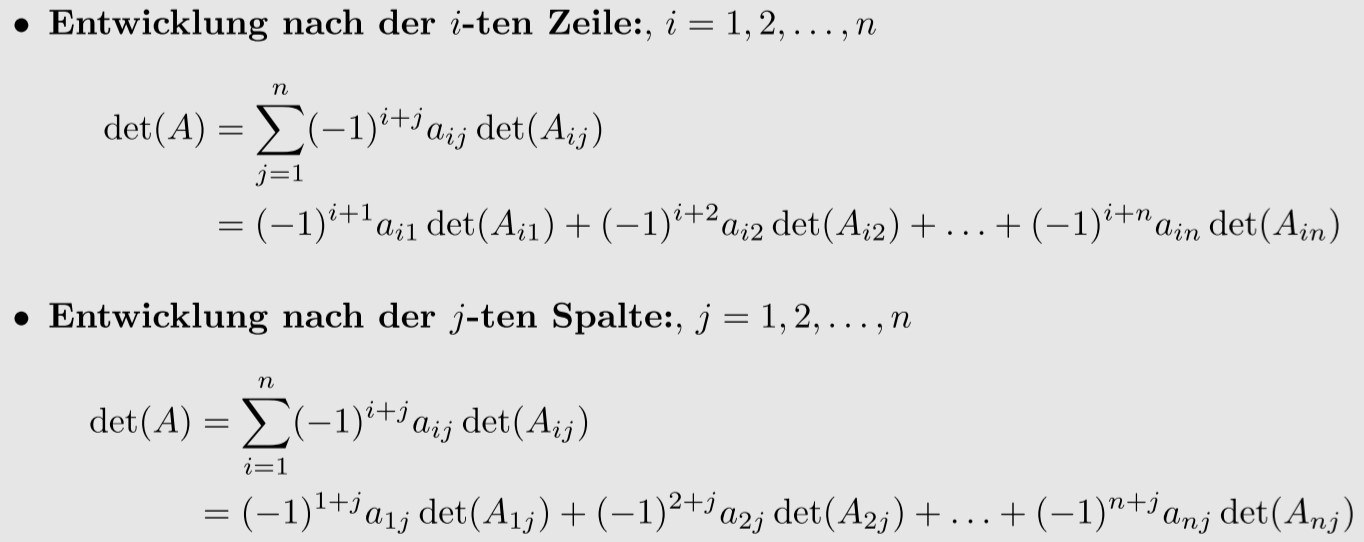
\includegraphics[scale=0.255]{laplacescher-entwicklungssatz}

\textbf{Anmerkung:}
\begin{itemize}
    \item Der Wert der Determinante ist \textbf{unabhängig} von der Entwicklungszeile oder -spalte.
    \item Es wird nach derjenigen Zeile/Spalte entwickelt, die die meisten Nullen enthält.
    \item Der Vorzeichenfaktor kann wiederum nach der Schachbrettregel bestimmt werden.
\end{itemize}
\vspace{-0.7em}
\begin{center}
    \begin{tabular}{|c|c|c|}
        \hline
        + & - & + \\
        \hline
        - & + & - \\
        \hline
        + & - & + \\
        \hline
    \end{tabular}
\end{center}
\vspace{-0.7em}

\ssect{Determinanten und LGS}

Die folgenden Aussagen sind äquivalent:
\begin{itemize}
    \item $\det(A) = 0$
    \item Der Rang von $A$ ist kleiner als $n$: $\text{rang}(A) < n$
    \item Das LGS $A \vec{x} = \vec{b}$ hat keine eindeutige Lösung.
    \item Die Matrix $A$ ist nicht invertierbar.
\end{itemize}

Die folgenden Aussagen sind ebenfalls äquivalent:
\begin{itemize}
    \item $\det(A) \neq 0$
    \item Der Rang von $A$ ist gleich $n$: $\text{rang}(A) = n$
    \item Das LGS $A \vec{x} = \vec{b}$ hat genau eine Lösung: $\vec{x} = A^{-1}\vec{b}$
    \item Die Matrix $A$ ist invertierbar.
\end{itemize}

\sssect{Geometrische Interpretation}

Der Betrag einer Determinante entspricht
\begin{itemize}
    \item dem \textbf{Flächeninhalt} einer $2 \times 2$ Matrix
    \item dem \textbf{Volumen} einer $3 \times 3$ Matrix
\end{itemize}
\[A = |\vec{a} \times \vec{b}| = \left| \det \left(
\begin{array}{cc}
    a_1 & b_1 \\
    a_2 & b_2
\end{array}
\right)\right|\]

        \sect{Vektoren}

\ssect{Definition}

Ein Vektor ist ein Object mit \textbf{Betrag} und \textbf{Richtung} hat.

\ssect{Operationen}

\sssect{Addition}

\begin{multicols}{2}
    \[\vec{a} + \vec{b} = \left(
    \begin{array}{c}
        a_x + b_x \\
        a_y + b_y
    \end{array}
    \right)\]
    \begin{center}
        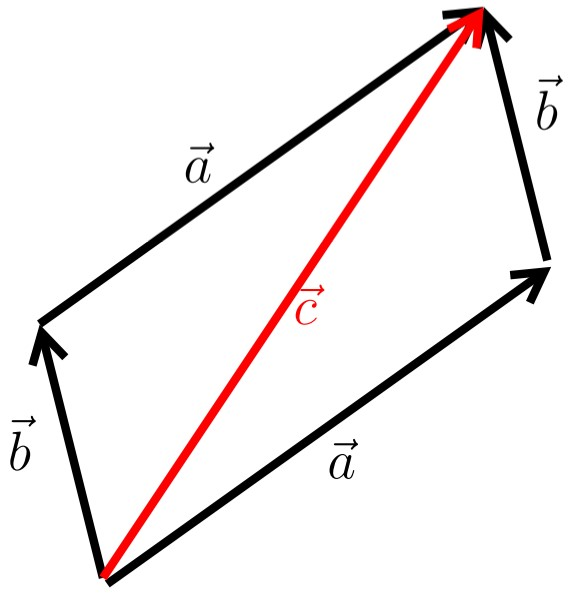
\includegraphics[scale=0.133]{vektor-addition}
    \end{center}
\end{multicols}

\textbf{Rechenregeln:}
\begin{enumerate}
    \item \textbf{Kommutativgesetz:} $\vec{a} + \vec{b} = \vec{b} + \vec{a}$
    \item \textbf{Assoziativgesetz:} $(\vec{a} + \vec{b}) + \vec{c} = \vec{a} + (\vec{b} + \vec{c})$
    \item Der Nullvektor ist das \textbf{Neutralelement}: $\vec{a} + \vec{0} = \vec{a}$
    \item Zu jedem Vektor $\vec{a}$ gibt es genau einen \textbf{Gegenvektor} $-\vec{a} \in \R^n$ mit $\vec{a} + (-\vec{a}) = \vec{0}$
\end{enumerate}

\sssect{Skalare Multiplikation}

\vspace{0.5em}

\begin{multicols}{2}
    \[\lambda \cdot \vec{a} = \left(
    \begin{array}{c}
        \lambda \cdot \vec{a_x} \\
        \lambda \cdot \vec{a_y}
    \end{array}
    \right)\]

    $\vec{a}$ und $\vec{b}$ heissen \textbf{kollinear}, falls $\vec{a} = \lambda \vec{b}$.
    Andernfalls heissen sie \textbf{windschief}.
\end{multicols}

Seien $\vec{w}_1, \dots, \vec{w}_m$ Vektoren und $a_1, \dots, a_m$ reellen Zahlen mit $m \in \N$.
Der Vektor \[\vec{v} = a_1 \vec{w}_1 + \dots + a_m \vec{w}_m \coloneqq \sum_{i=1}^{m} a_i \vec{w}_i\] heisst eine \textbf{Linearkombination} von den Vektoren.
Die Zahlen $a_1, \dots, a_m$ heissen \textbf{Koeffizienten}.

\sssect{Betrag}

\vspace{0.5em}

\begin{multicols}{2}
    \begin{center}
        $|\vec{a}| = \sqrt{a_x^2 + a_y^2 + a_z^2}$
    \end{center}

    \textbf{Einheitsvektor}: $|\vec{e}| = 1$
\end{multicols}

\sssect{Skalarprodukt}

Das \textbf{Skalarprodukt} (Engl.\ dot product) berechnet sich aus:
\begin{itemize}
    \item $\vec{a} \cdot \vec{b} = |\vec{a}| |\vec{b}| \cos(\varphi)$
    \item $\vec{a} \cdot \vec{b} = |\vec{a}|^2$
    \item $\vec{a} \cdot \vec{b} = a_1 b_1 + \dots + a_n b_n = \sum_{i=1}^{n} a_i b_i$
\end{itemize}

\textbf{Anmerkung:}
\begin{itemize}
    \item Das Skalarprodukt wird auch als $(\vec{a}, \vec{b})$, $\langle \vec{a} | \vec{b} \rangle$ oder $\vec{a}^T \vec{b}$ geschrieben.
    \item Der Winkel $\varphi$ ist stets \textbf{der kleinere} der beiden Winkel zwischen den Vektoren: $0^{\circ} \leq \varphi \leq 180^{\circ}$
\end{itemize}

Zwei Vektoren sind \textbf{orthogonal} zueinander, falls: \[\vec{a} \cdot \vec{b} = 0 \Leftrightarrow \vec{a} \perp \vec{b}\]

Der Winkel zwischen zwei Vektoren berechnet sich aus: \[\varphi = \arccos \left( \frac{\vec{a} \cdot \vec{b}}{|\vec{a}| |\vec{b}|} \right)\]

\sssect{Vektorprodukt}

\begin{itemize}
    \item $|\vec{a} \times \vec{b}| = |\vec{a}| \cdot |\vec{b}| \sin(\varphi)$
    \item $\vec{a} \times \vec{b}$ \textbf{ist orthogonal zu $\vec{a}$ und $\vec{b}$}
    \item $\vec{a} \times \vec{b} \neq \vec{b} \times \vec{a}$
\end{itemize}
\[\vec{a} \times \vec{b} = \left(
\begin{array}{c}
    a_x \\ a_y \\ a_z
\end{array}
\right) \times \left(
\begin{array}{c}
    b_x \\ b_y \\ b_z
\end{array}
\right) = \left(
\begin{array}{c}
    a_y b_z - a_z b_y \\
    a_z b_x - a_x b_z \\
    a_x b_y - a_y b_x
\end{array}
\right)\]
\textbf{Anmerkung:}
\begin{itemize}
    \item Das Vektorprodukt ist im Gegensatz zum Skalarprodukt eine \textbf{vektorielle Grösse} und wird auch als \textbf{äusseres Produkt} oder \textbf{Kreuzprodukt} bezeichnet.
    \item Das Vektorprodukt existiert im Gegensatz zum Skalarprodukt \textbf{nur} für dreidimensionale Vektoren.
    \item Der Betrag des Vektorproduktes entspricht dem \textbf{Flächeninhalt} des von den Vektoren $\vec{a}$ und $\vec{b}$ aufgespannten Parallelogramms.
    \item $\vec{a} \times \vec{b} = 0 \Leftrightarrow$ $\vec{a}$ und $\vec{b}$ sind \textbf{kollinear}
    \item $\vec{a} \times \vec{b} = -(\vec{b} \times \vec{a})$
\end{itemize}
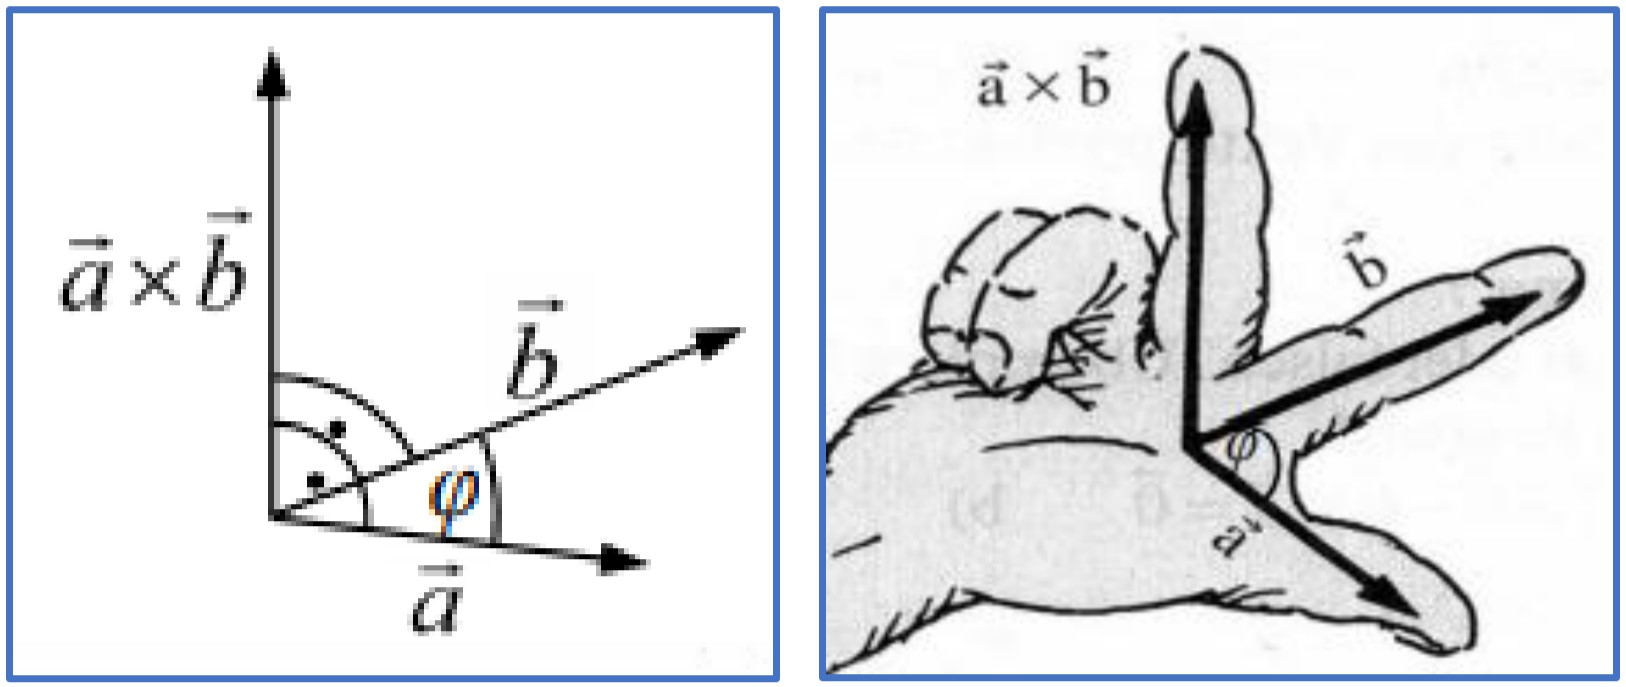
\includegraphics[scale=0.21]{vektorprodukt}

\sssect{Komplanar}

$\vec{a}$, $\vec{b}$ und $\vec{c}$ heissen \textbf{komplanar}, wenn sie auf gleichen Ebene liegen.
$\vec{a}$ lässt sich dann als Linearkombination von $\vec{b}$ und $\vec{c}$ ausdrücken:
\[\vec{a} = \lambda \vec{b} + \mu \vec{c}\]

\begin{center}
    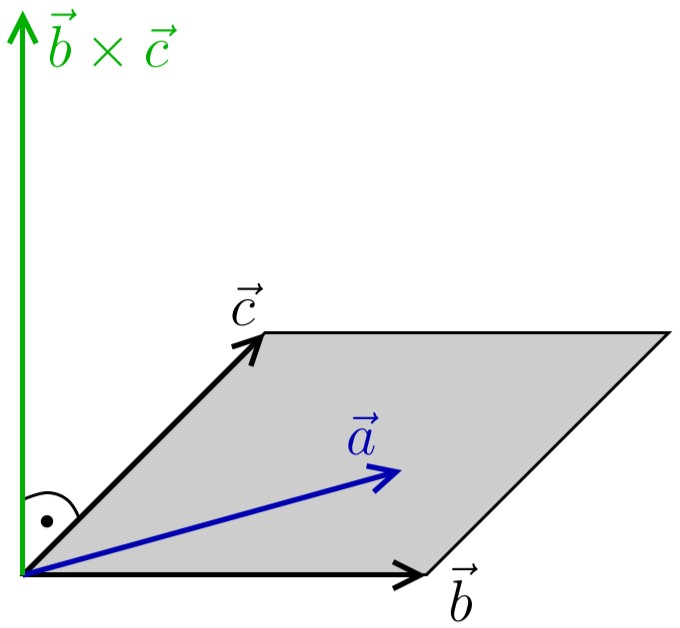
\includegraphics[scale=0.18]{komplanar}
\end{center}

\ssect{Geraden}

\sssect{Parametergleichung}

\vspace{0.5em}
\begin{multicols}{2}
    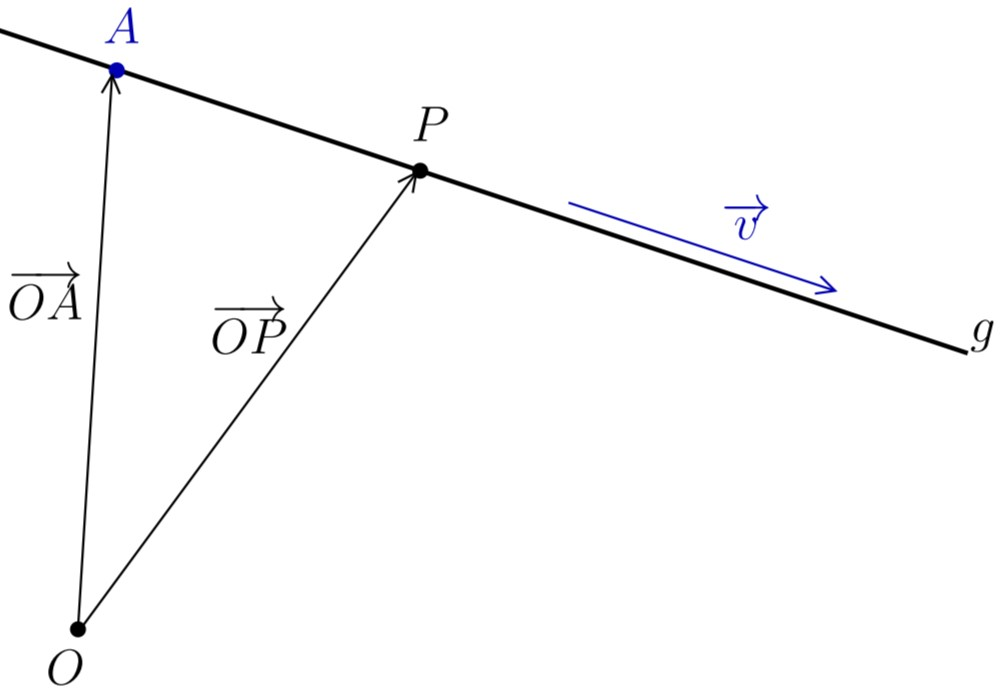
\includegraphics[scale=0.15]{parametergleichung-gerade}

    $g$ sei eine Gerade, die durch den Punkt $A$ und parallel zum Richtungsvektor $\vec{v}$ verläuft.
    Eine \textbf{Parameterdarstellung} dieser Geraden lautet:
    $g: \vec{OA} + \lambda \vec{v}$
\end{multicols}

Der Punkt $A$ heisst \textbf{Aufpunkt}, der Vektor $\vec{OA}$ heisst \textbf{Stützvektor} und der Vektor $\vec{v}$ heisst \textbf{Richtungsvektor}.

Ein Punkt $P$ liegt genau dann auf $g$, wenn es ein $\lambda$ gibt, sodass gilt:
$\vec{OP} = \vec{OA} + \lambda \vec{v}$

\sssect{Koordinatengleichung}

\begin{center}
    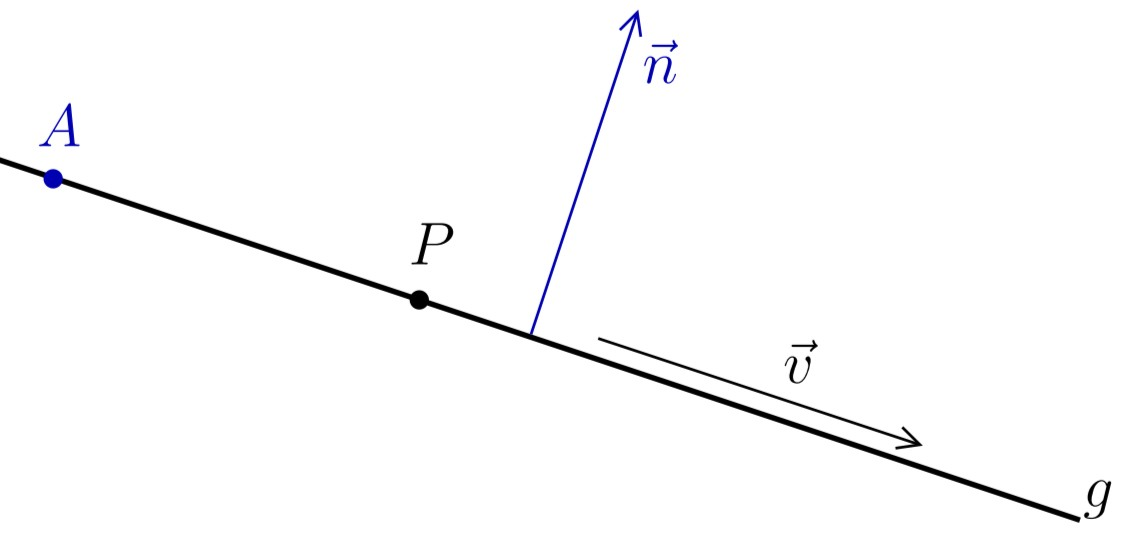
\includegraphics[scale=0.17]{koordinatengleichung-gerade}
\end{center}

$g$ sei eine Gerade, die durch den Punkt $A = (a_x, a_y)$ und senkrecht zum Normalenvektor $n = (a \ b)^T$ verläuft.
Die \textbf{Koordinatengleichung} lautet:
\[\vec{n} \cdot \vec{OP} - n \cdot \vec{OA} = 0\]
Oder in der Komponentenschreibweise:
\[ax + by + c = 0\]
wobei $c = -\vec{n} \cdot \vec{OA} = -(a a_x + b a_y)$ und $P = (x, y)$.

\textbf{Beispiel:} $A = (4 \ 6)^T$ und $\vec{n} = (3 \ -1)^T$
\[g: 3x - y - (3 \cdot 4 - 1 \cdot 6) = 0 \Leftrightarrow 3x - y - 6 = 0\]


\sssect{Gegenseitige Lage in der Ebene}

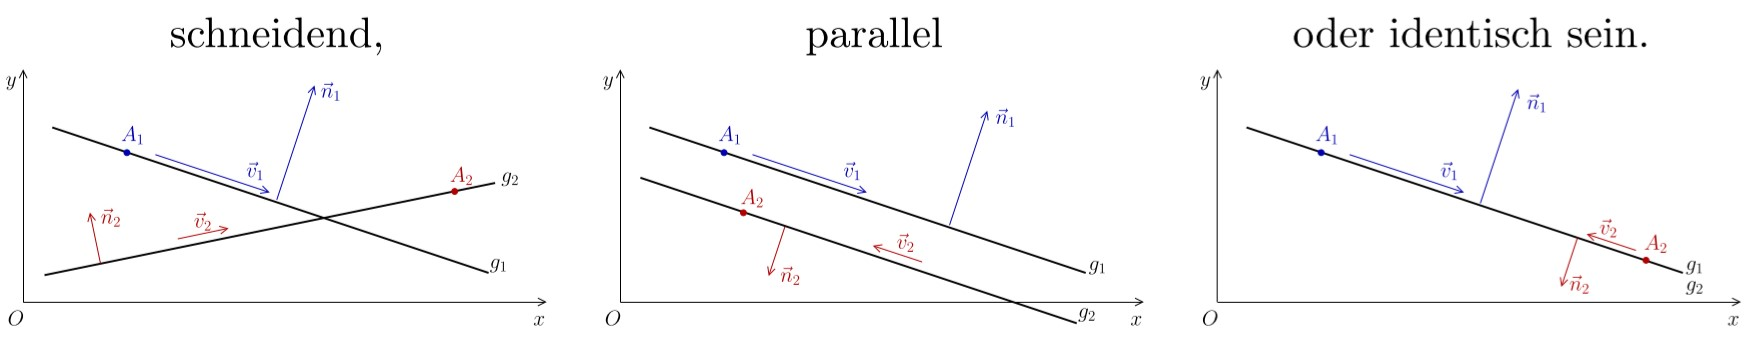
\includegraphics[scale=0.2]{gegenseitige-lage-geraden-ebene}

\sssect{Gegenseitige Lage im Raum}

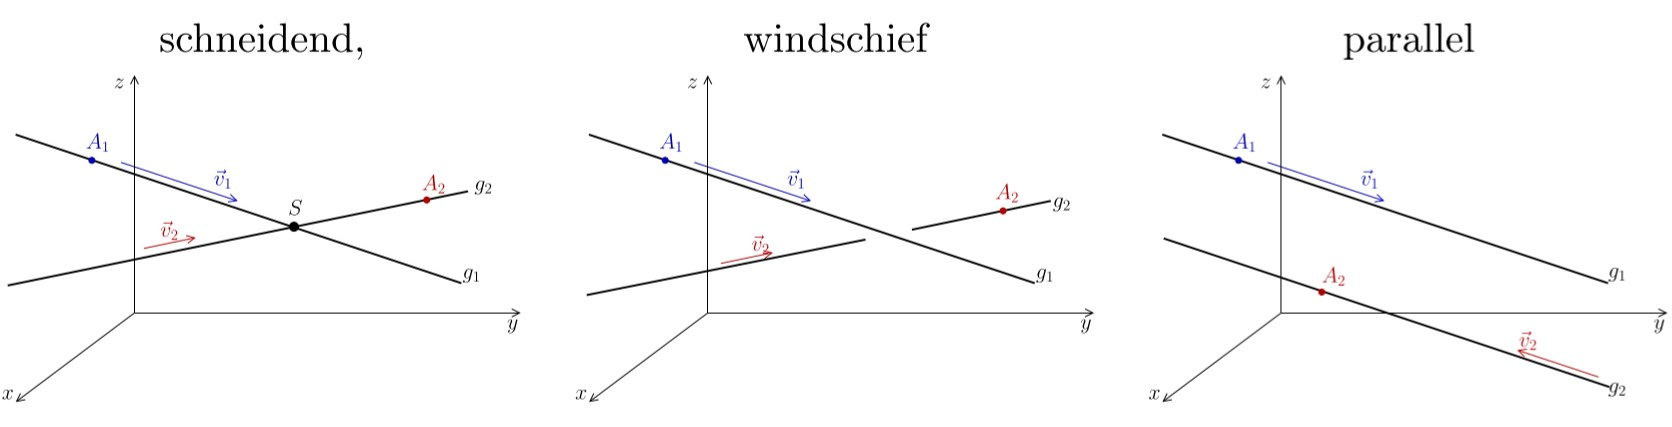
\includegraphics[scale=0.21]{gegenseitige-lage-geraden-raum}

\ssect{Ebenen}

\sssect{Parametergleichung}

\vspace{0.5em}
\begin{multicols}{2}
    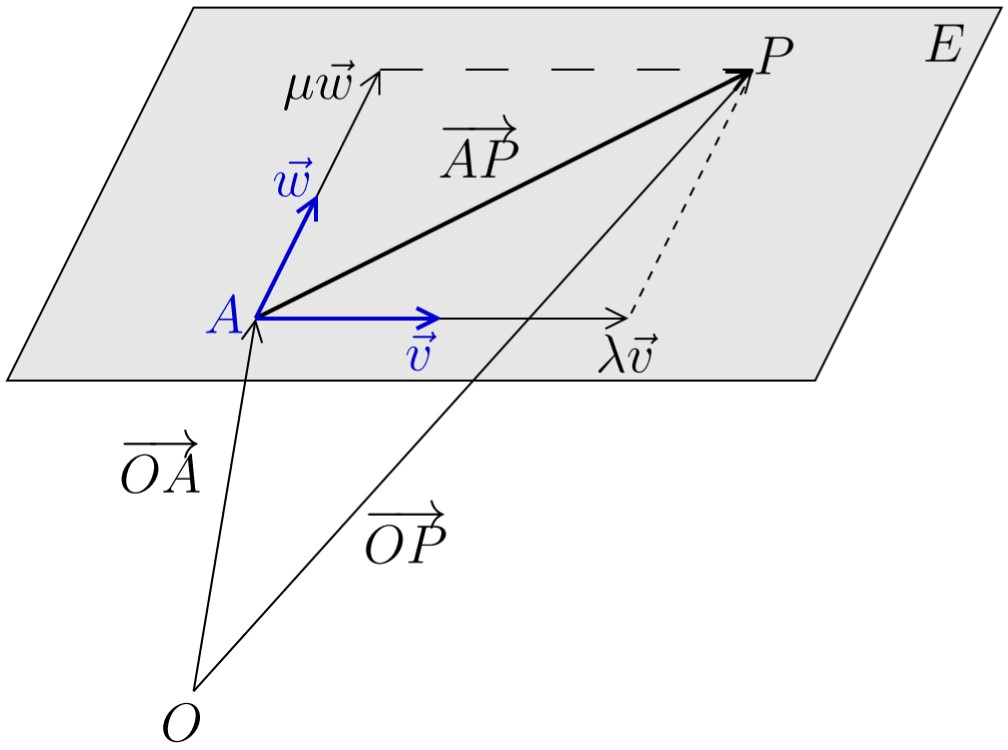
\includegraphics[scale=0.17]{parametergleichung-ebene}

    $E$ sei eine Ebene, die durch den Punkt $A$ und parallel zu zwei nichtkollinearen Vektoren $\vec{v}$ und $\vec{w}$ verläuft.
    Die \textbf{vektorielle Parameterform} der Ebene-Gleichung lautet:
    \[\vec{OP} = \vec{OA} + \lambda \vec{v} + \mu \vec{w}\]
\end{multicols}

$\vec{v}$ und $\vec{w}$ heissen \textbf{Richtungsvektoren} der Ebene $E$.

\sssect{Koordinatengleichung}

Ein auf der Ebene $E$ senkrecht stehender Vektor $\vec{n}$ heisst \textbf{Normalenvektor der Ebene}: $\vec{n} = \vec{v} \times \vec{w}$

\vspace{0.5em}
\begin{multicols}{2}
    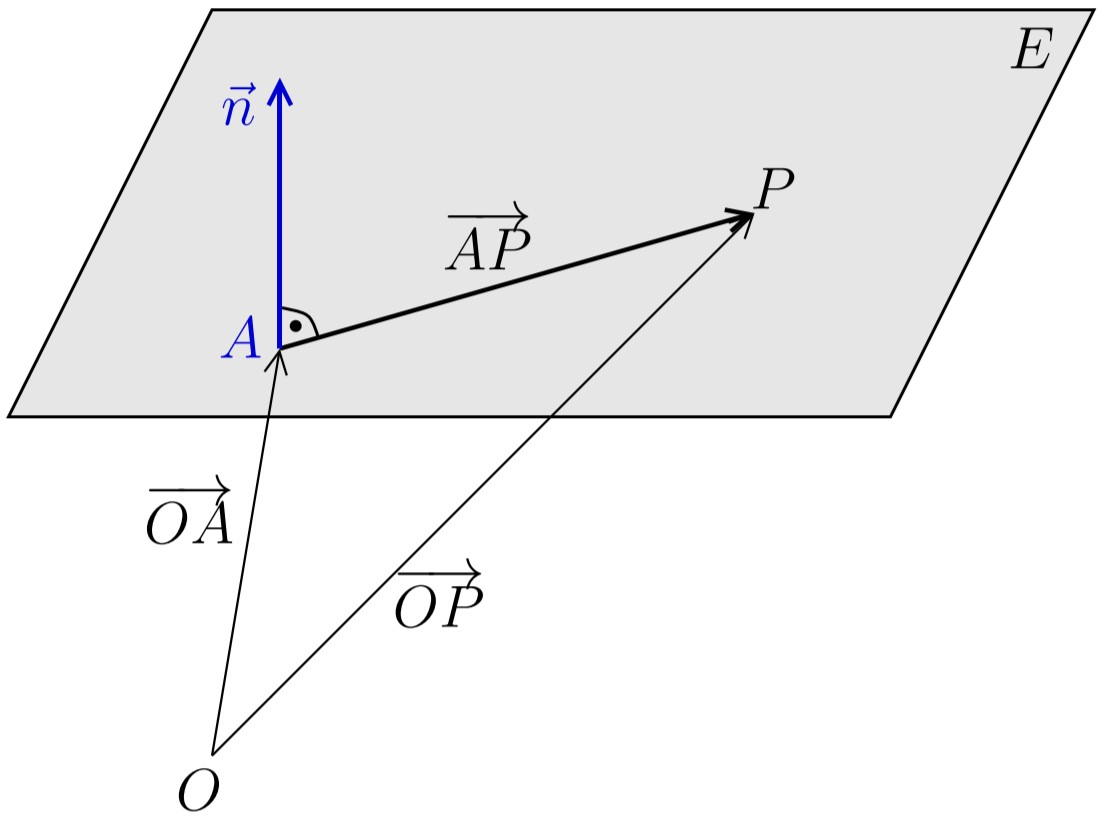
\includegraphics[scale=0.15]{koordinatengleichung-ebene}

    $E$ sei eine Ebene, die durch den Punkt $A = (a_x, a_y, a_z)$ und senkrecht zum Normalenvektor $n = (a \ b \ c)^T$ verläuft.
    Die \textbf{Koordinatengleichung} lautet:
    \[E: \vec{n} \cdot (\vec{OP} - \vec{OA}) = 0\]
\end{multicols}

Oder in der Komponentenschreibweise:
\[E: ax + by + cz + d = 0\]
wobei $d = -\vec{n} \cdot \vec{OA} = -(a a_x + b a_y + c a_z)$ und $P = (x, y, z)$.

\textbf{Beispiel:} $A = (2 \ -5 \ 3)^T$ und $\vec{n} = (4 \ 2 \ 5)$
\[4x + 2y + 5z - (4 \cdot 2 + 2 \cdot (-5) + 5 \cdot 3) = 0 \Leftrightarrow 4x + 2y + 5z - 13 = 0\]
Der Punkt $Q(0; 4; 1)$ gehört zur Ebene, da
\[4 \cdot 0 + 2 \cdot 4 + 5 \cdot 1 - 13 = 8 + 5 - 13 = 0\]

\sssect{Gegenseitige Lage im Raum}

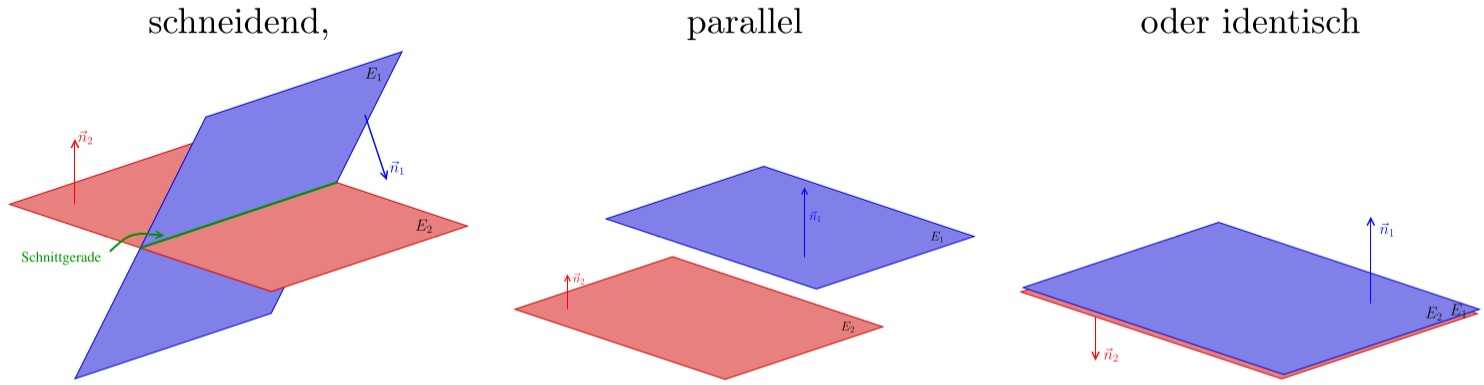
\includegraphics[scale=0.23]{gegenseitige-lage-ebenen-raum}

\ssect{Abständen}

\sssect{Abstand Punkt-Gerade in der Ebene}

\begin{center}
    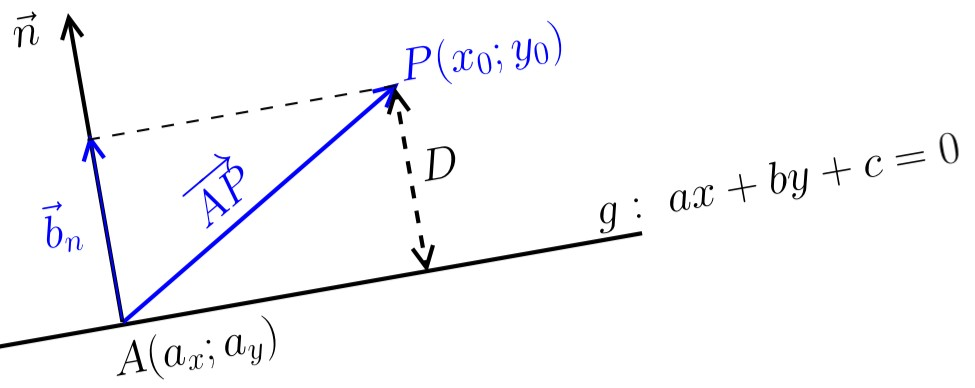
\includegraphics[scale=0.22]{abstand-punkt-gerade-ebene}
\end{center}

Der Abstand $D$ eines beliebigen Punktes $P(x_0, y_0)$ von der Geraden $g: ax + by + c = 0$ berechnet sich aus:
\[D = \frac{|\vec{AP} \cdot \vec{n}|}{|\vec{n}|} = \frac{|a x_0 + b y_0 + c|}{\sqrt{a^2 + b^2}}\]

\textbf{Beispiel:} Abstand des Punktes $P(5;7)$ von der Gerade $g: 3x + 4y + 15 = 0$:
\[D = \frac{|3 \cdot 5 + 4 \cdot (-7) + 15|}{\sqrt{3^2 + 4^2}} = \frac{|15 - 28 + 15|}{\sqrt{25}} = \frac{2}{5}\]

\sssect{Abstand Punkt-Gerade im Raum}

\begin{center}
    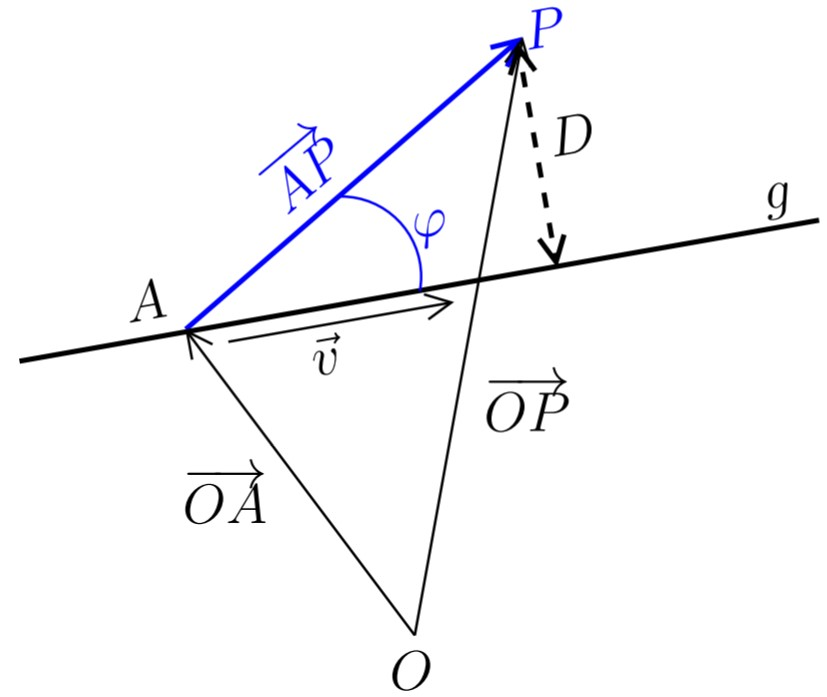
\includegraphics[scale=0.18]{abstand-punkt-gerade-raum}
\end{center}

Der Abstand $D$ eines beliebigen Punktes $P$ von der Geraden $g: \vec{OA} + \lambda \vec{v}$ berechnet sich aus:
\[D = \frac{|\vec{v} \times \vec{AP}|}{|\vec{v}|}\]

\textbf{Beispiel:}
Die Parametergleichung einer Geraden $g$ lautet:
\[g: \vec{OA} + \lambda \vec{v} = \left(
\begin{array}{c}
    1 \\ 0 \\ 1
\end{array}
\right) + \lambda \left(
\begin{array}{c}
    2 \\ 5 \\ 2
\end{array}
\right)\]
Wir berechnen den Abstand $D$ von $P(5;3;-2)$ zu $g$.
Zuerst berechnen wir das Vektorprodukt $\vec{v} \times \vec{AP}$:
\[\vec{v} \times \vec{AP} = \left(
\begin{array}{c}
    2 \\ 5 \\ 2
\end{array}
\right) \times \left(
\begin{array}{c}
    5 - 1 \\
    3 - 0 \\
    -2 - 1
\end{array}
\right) = \left(
\begin{array}{c}
    2 \\ 5 \\ 2
\end{array}
\right) \times \left(
\begin{array}{c}
    4 \\ 3 \\ -3
\end{array}
\right) = \left(
\begin{array}{c}
    -21 \\ 14 \\ -14
\end{array}
\right)\]
Daraus folgt:
\[|\vec{v} \times \vec{AP}| = \sqrt{(-21)^2 + 14^2 + (-14)^2} = \sqrt{833}\]
Wir müssen noch den Betrag von $\vec{v}$ berechnen:
\[|\vec{v}| = \sqrt{2^2 + 5^2 + 2^2} = \sqrt{33}\]
Somit: $D = \frac{|\vec{v} \times \vec{AP}|}{|\vec{v}|} = \frac{\sqrt{833}}{\sqrt{33}} \approx 5.02$

\sssect{Abstand Punkt-Ebene}

\begin{center}
    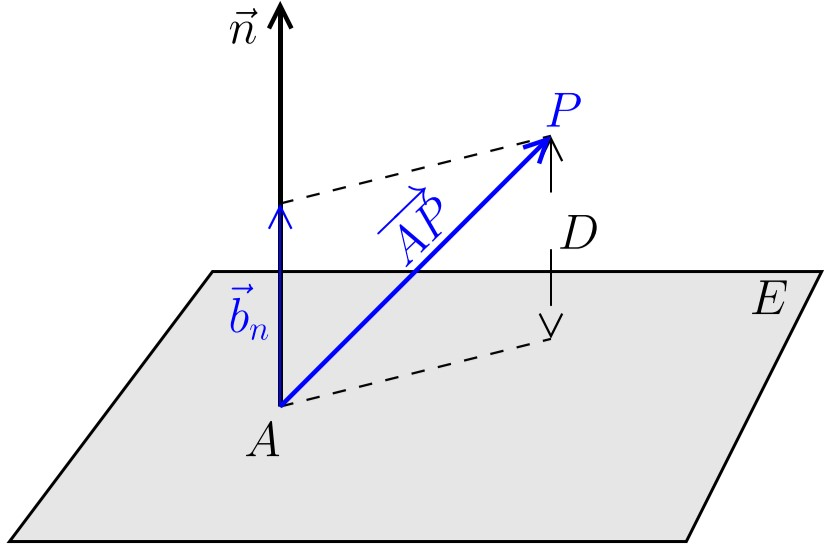
\includegraphics[scale=0.18]{abstand-punkt-ebene}
\end{center}

Der Abstand $D$ eines beliebigen Punktes $P(x_0, y_0, z_0)$ von der Ebene $E: ax + by + cz + d = 0$ berechnet sich aus:
\[D = \frac{|\vec{AP} \cdot \vec{n}|}{|\vec{n}|} = \frac{|a x_0 + b y_0 + c z_0 + d|}{\sqrt{a^2 + b^2 + c^2}}\]

\textbf{Beispiel:} Abstand von Punkt $P(1;0;-2)$ und der Ebene $E\colon -2x + y - 3z - 18 = 0$:
\[D = \frac{|-2 \cdot 1 + 1 \cdot 0 - 3 \cdot (-2) -18|}{\sqrt{(-2)^2 + 1^2 + (-3)^2}} = \frac{|-14|}{\sqrt{14}} = \frac{14}{\sqrt{14}} \approx 3.74\]

        \sect{Vektorräume}

\ssect{Definition}

Ein \textbf{reeller Vektorraum} besteht aus einer nichtleeren Menge $\V$ von Elementen, die wir Vektoren nennen.
Auf der Menge $\V$ gibt es die folgenden Vorschriften:
\begin{itemize}
    \item Die \textbf{Addition}: Für alle Vektoren $\vec{a}$ und $\vec{b}$ in $\V$ ist der Vektor $\vec{a} + \vec{b}$ wieder in $\V$.
    \item Die \textbf{skalare Multiplikation}: Für alle Vektoren $\vec{a} \in \V$ und alle Skalare $\lambda \in \R$ ist der Vektor $\lambda \vec{a}$ wieder in $\V$.
\end{itemize}
Ferner sollen für alle Vektoren $\vec{a}, \vec{b}, \vec{c}$ aus $\V$ und alle Skalare $\lambda, \mu$ aus $\R$ folgende acht Rechengesetze gelten:
\begin{enumerate}
    \item \textbf{Kommutativität} für die Addition: $\vec{a} + \vec{b} = \vec{b} + \vec{a}$
    \item \textbf{Assoziativität} für die Addition: $\vec{a} + (\vec{b} + \vec{c}) = (\vec{a} + \vec{b}) + \vec{c}$
    \item \textbf{Neutralelement} der Addition $\vec{0}$: $\vec{a} + \vec{0} = \vec{a}$
    \item Existenz \textbf{entgegengesetzter Elemente}: Zu jedem $\vec{a} \in \V$ gibt es genau ein entgegengesetztes Element $-\vec{a} \in \V$ mit $\vec{a} + (-\vec{a}) = \vec{0}$
    \item \textbf{Distributivität}: $\lambda (\vec{a} + \vec{b}) = \lambda \vec{a} + \lambda \vec{b}$
    \item \textbf{Distributivität}: $(\lambda + \mu) \vec{a} = \lambda \vec{a} + \mu \vec{a}$
    \item \textbf{Assoziativität} für die Multiplikation: $\lambda (\mu \vec{a}) = (\lambda \mu) \vec{a}$
    \item Die reelle Zahl 1 ist das \textbf{Neutralelement} der skalaren Multiplikation: $1 \cdot \vec{a} = \vec{a}$
\end{enumerate}

\sssect{Unterraum}

$V$ sei ein Vektorraum und $U$ eine nichtleere Teilmenge von $V$.
Ist $U$ ein Vektorraum bzgl.\ der Addition und skalaren Multiplikation in $V$, so ist $U$ ein \textbf{Unterraum} von $V$.

\textbf{Satz Unterraumkriterium:} Es sei $V$ ein Vektorraum und $U$ eine nichtleere Teilmenge von $V$.
$U$ ist genau dann ein \textbf{Unterraum von $V$}, wenn die beiden folgenden Bedingungen erfüllt sind:
\begin{itemize}
    \item $\vec{a} + \vec{b} \in U$ mit $\forall \vec{a}, \vec{b} \in U$
    \item $\lambda \vec{a} \in U$ mit $\forall \vec{a} \in U, \forall \lambda \in \R$
\end{itemize}

Es gilt:
\begin{itemize}
    \item Eine Ebene ist genau dann ein Unterraum von $\R^3$, wenn sie den Ursprung enthält.
    \item Eine durch den Ursprung gehende Gerade in $\R^2$ ist ein Unterraum von $\R^2$.
    \item Das Neutralelement muss zu jedem Unterraum gehören.
\end{itemize}

\ssect{Lineare Hülle}

Sei $V$ ein Vektorraum und seien $\vec{v}_1, \dots, \vec{v}_n \in V$.
Die Menge aller Linearkombinationen der Vektoren $\vec{v}_1, \dots, \vec{v}_n$ ist
\[\text{Lin}(\vec{v}_1, \dots, \vec{v}_n) = \{ \vec{x} \in V \mid \vec{x} = \lambda_1 \vec{v}_1 + \dots + \lambda_n \vec{v}_n\}\]
und heisst \textbf{lineare Hülle} (auch der \textbf{Spann}) der Vektoren $\vec{v}_1, \dots, \vec{v}_n$.
Man sagt auch, dass $\vec{v}_1, \dots, \vec{v}_n$ die Menge $\text{Lin}(\vec{v}_1, \dots, \vec{v}_n)$ erzeugen, oder dass $\vec{v}_1, \dots, \vec{v}_n$ ein \textbf{Erzeugendensystem} von $\text{Lin}(\vec{v}_1, \dots, \vec{v}_n)$ bilden.

\textbf{Anmerkung:} Die lineare Hülle der Vektoren $\vec{v}_1, \dots, \vec{v}_n \in V$ lässt sich auch als $Span(\vec{v}_1, \dots, \vec{v}_n)$ schreiben.

\textbf{Satz:} Sei $V$ ein Vektorraum und seien $\vec{v}_1, \dots, \vec{v}_n \in V$.
Die Menge $\text{Lin}(\vec{v}_1, \dots, \vec{v}_n)$ ist ein Unterraum von $V$.

\ssect{Lineare Abhängigkeit/Unabhängigkeit}

Eine Familie von Vektoren $\vec{v}_1, \dots, \vec{v}_m$ heissen \textbf{linear unabhängig}, wenn die folgende Vektorgleichung \[\lambda_1 \vec{v}_1 + \dots + \lambda_m \vec{v}_m = \vec{0}\] nur für verschwindende Koeffizienten $\lambda_1, \dots, \lambda_m \in \R$ erfüllt werden kann.
Andernfalls heissen die $m$ Vektoren \textbf{linear abhängig}, d.h.\ es ist mind.\ ein Koeffizient ungleich Null.

Es gelten:
\begin{itemize}
    \item $\vec{a}_1, \dots, \vec{a}_n \in \R^n \text{ linear abhängig } \Leftrightarrow \det(A) = 0$
    \item $\vec{a}_1, \dots, \vec{a}_n \in \R^n \text{ linear unabhängig } \Leftrightarrow \det(A) \neq 0$
\end{itemize}

\textbf{Verfahren zur Bestimmung, ob Vektoren linear abhängig sind oder nicht:}
\begin{enumerate}
    \item Man bildet die folgende erweiterte Koeffizientenmatrix:
    \[(\vec{a}_1 \ \dots \ \vec{a}_n \mid \vec{0}) = \left(
    \begin{array}{ccc|c}
        a_{11} & \ldots & a_{1n} & 0      \\
        \vdots & \ddots & \vdots & \vdots \\
        a_{m1} & \ldots & a_{mn} & 0
    \end{array}
    \right)\]
    \item Man bringt diese Matrix mit Gauss-Verfahren auf ZSF.\
    \item Hat die erweiterte Koeffizientenmatrix auf ZSF nur führende Variablen (d.h.\ ist der Rang der Matrix gleich $n$), dann hat das System genau eine Lösung und die Vektoren sind \textbf{linear unabhängig}.\\
    Besitzt die erweiterte Koeffizientenmatrix auf ZSF freie Variablen (d.h.\ ist der Rang der Matrix kleiner als $n$), dann hat das System unendlich viele Lösungen.
    Somit die Vektoren \textbf{linear abhängig}.
\end{enumerate}

\ssect{Basis und Dimension}

Die Vektoren $\vec{v}_1, \dots, \vec{v}_n \in V$ bilden eine \textbf{Basis} $\B = \{ \vec{v}_1, \dots, \vec{v}_n \}$ des Vektorraums $V$, wenn gilt:
\begin{itemize}
    \item Die Vektoren sind linear unabhängig.
    \item $\text{Lin}(\vec{v}_1, \dots, \vec{v}_n) = V$, d.h.\ jeder Vektor lässt sich als Linearkombination der Vektoren $\vec{v}_1, \dots, \vec{v}_n$ darstellen: \[\vec{v} = \lambda_1 \vec{v}_1 + \dots + \lambda_n \vec{v}_n\]
\end{itemize}
Die Vektoren $\vec{v}_1, \dots, \vec{v}_n$ heissen \textbf{Basisvektoren} und die Skalare $\lambda_1, \dots, \lambda_n$ sind die \textbf{Koordinaten von $\vec{v}$ bezüglich der Basis $\B$}.

\textbf{Anmerkung:}
\begin{itemize}
    \item Die Koordinaten $\lambda_1, \dots, \lambda_n$ sind eindeutig bestimmt, d.h.\ es gibt genau einen $\lambda_1, \dots, \lambda_n$, sodass gilt: \[\vec{v} = \lambda_1 \vec{v}_1 + \dots + \lambda_n \vec{v}_n\]
    \item Ein Erzeugendensystem eines Vektorraumes kann linear abhängige oder unabhängige Vektoren enthalten.
    Eine Basis ist ein Erzeugendensystem, bei dem alle Vektoren \textbf{linear unabhängig} sind.
    \item Die Basis eines Vektorraumes ist \textbf{nicht eindeutig}, d.h.\ es gibt verschiedene Basen in einem Vektorraum.
\end{itemize}

Die Anzahl der Vektoren einer Basis eines Vektorraumes $V$ ist die \textbf{Dimension} des Vektorraumes.
Hierfür schreiben wir $\dim(V)$.

\textbf{Satz:} Wir betrachten die Vektoren $\vec{a}_1, \dots, \vec{a}_n \in \R^n$ sowie die $n \times n$ Matrix $A$, die entsteht, wenn wir die Vektoren nebeneinander schreiben.
Die folgenden Aussagen sind äquivalent:
\begin{itemize}
    \item Die Vektoren $\vec{a}_1, \dots, \vec{a}_n$ bilden eine Basis von $\R^n$
    \item $\text{rang}(A) = n$
    \item $\det(A) \neq 0$
    \item $A$ ist invertierbar
    \item Das LGS $A \vec{x} = \vec{b}$ hat eine eindeutige Lösung
\end{itemize}

\textbf{Beispiel:} Folgende Matrizen bilden eine Basis für $\R^{2 \times 2}$:
\[A_1 = \left(
\begin{array}{cc}
    1 & 0 \\ 0 & 0
\end{array}
\right), A_2 = \left(
\begin{array}{cc}
    0 & 1 \\ 0 & 0
\end{array}
\right), A_3 = \left(
\begin{array}{cc}
    0 & 0 \\ 1 & 0
\end{array}
\right), A_4 = \left(
\begin{array}{cc}
    0 & 0 \\ 0 & 1
\end{array}
\right)\]
Es gilt nämlich:
\begin{itemize}
    \item Diese Matrizen sind linear unabhängig:
    \begin{align*}
        \lambda_1 A_1 + \lambda_2 A_2 + \lambda_3 A_3 + \lambda_4 A4 &= 0 \\
        \left(
        \begin{array}{cc}
            \lambda_1 & 0 \\ 0 & 0
        \end{array}
        \right) + \left(
        \begin{array}{cc}
            0 & \lambda_2 \\ 0 & 0
        \end{array}
        \right) + \left(
        \begin{array}{cc}
            0 & 0 \\ \lambda_3 & 0
        \end{array}
        \right) + \left(
        \begin{array}{cc}
            0 & 0 \\ 0 & \lambda_4
        \end{array}
        \right) &= \left(
        \begin{array}{cc}
            0 & 0 \\ 0 & 0
        \end{array}
        \right) \\
        \left(
        \begin{array}{cc}
            \lambda_1 & \lambda_2 \\ \lambda_3 & \lambda_4
        \end{array}
        \right) &= \left(
        \begin{array}{cc}
            0 & 0 \\ 0 & 0
        \end{array}
        \right) \\
        \Rightarrow \lambda_1 = \lambda_2 = \lambda_3 = \lambda_4 &= 0
    \end{align*}
    \item Für eine beliebige Matrix $A = \left(
    \begin{array}{cc}
        a_{11} & a_{12} \\
        a_{21} & a_{22}
    \end{array}
    \right)$ gilt:
    \begin{align*}
        A &= \left(
        \begin{array}{cc}
            a_{11} & 0 \\
            0      & 0
        \end{array}
        \right) + \left(
        \begin{array}{cc}
            0 & a_{12} \\
            0 & 0
        \end{array}
        \right) + \left(
        \begin{array}{cc}
            0      & 0 \\
            a_{21} & 0
        \end{array}
        \right) + \left(
        \begin{array}{cc}
            0 & 0      \\
            0 & a_{22}
        \end{array}
        \right) \\
        &= a_{11} A_1 + a_{12} A_2 + a_{21} A_3 + a_{22} A_4
    \end{align*}
    Das heisst, dass $A$ sich als Linearkombination von $A_1, \dots, A_4$ darstellen lässt.
\end{itemize}

\ssect{Koordinatenvektor}

Seien $V$ ein reeller Vektorraum und $\B = \{\vec{v}_1, \dots, \vec{v}_n\}$ eine Basis von $V$.
Sei $\vec{v}$ ein beliebiger Vektor aus $V$ mit der Darstellung:
\[\vec{v} = \lambda_1 \vec{v}_1 + \dots + \lambda_n \vec{v}_n\]
wobei die eindeutig bestimmten Skalare $\lambda_1, \dots, \lambda_n$ die Koordinaten von $\vec{v}$ bezüglich $\B$ sind.
Dann nennt man den Vektor
\[\vec{v}_{\B} = \left(
\begin{array}{c}
    \lambda_1 \\ \vdots \\ \lambda_n
\end{array}
\right)_{\B}\]
den \textbf{Koordinatenvektor} oder die \textbf{Komponentendarstellung von $\vec{v}$ bezüglich $\B$}.

        \newpage

        \sect{Lineare Abbildungen}

\ssect{Definition}

Seien $V$ und $W$ zwei reelle Vektorräume und $f: V \rightarrow W$ eine Abbildung des Vektorraums $V$ in den Vektorraum $W$.
Die Abbildung $f$ ist eine \textbf{lineare Abbildung}, falls $\forall \vec{x}_1, \vec{x}_2 \in V$ und $\forall \lambda \in \R$ gilt:
\begin{itemize}
    \item $f(\vec{x}_1 + \vec{x}_2) = f(\vec{x}_1) + f(\vec{x}_2)$
    \item $f(\lambda \vec{x}_1) = \lambda f(\vec{x}_1)$
\end{itemize}

\textbf{Satz:} Für jede lineare Abbildung $f: V \rightarrow W$ gilt:
\begin{itemize}
    \item $f(-\vec{x}) = -f(\vec{x})$, $\forall \vec{x} \in V$.
    Das Bild des entgegengesetzten Vektors $-\vec{x}$ zum Vektor $\vec{x}$ ist immer gleich dem entgegengesetzten Element zum Bild von $\vec{x}$.
    \item $f(\vec{0}_V) = \vec{0}_W$, der Nullvektor $\vec{0}_V$ in $V$ wird immer in den Nullvektor $\vec{0}_W$ abgebildet.
\end{itemize}

\textbf{Satz:} Ist $\{ \vec{e}_1, \dots, \vec{e}_n \}$ die Standardbasis des $\R^n$ und ist eine beliebige Abbildung $f: \R^n \rightarrow \R^m$ gegeben, so bilden die Vektoren $\vec{a}_j \coloneqq f(\vec{e}_j) \in \R^m$ die Spalten einer Matrix $A \coloneqq (\vec{a}_1 \ \dots \ \vec{a}_n) \in \R^{m \times n}$ mit der Eigenschaft $A \vec{x} = f(\vec{x})$.
Man nennt diese Matrix die \textbf{Abbildungsmatrix}.

\textbf{Satz:} Wir betrachten zwei endlich-dimensionale Vektorräume $V$ mit Basis $\B = \{\vec{b}_1, \dots, \vec{b}_n$ und $W$ mit Basis $\C = \{\vec{c}_1, \dots, \vec{c}_m$.
Dann lässt sich jede lineare Abbildung $f: V \rightarrow W$ durch eine $m \times n$ Matrix ${}_{\C} A_{\B}$ darstellen:
\[\vec{y}_{\C} = (f(\vec{x}))_{\C} = {}_{\C} A_{\B} \vec{x}_{\B}\]
Die Spalten der Matrix ${}_{\C} A_{\B}$ sind die Bilder der Elemente von $\B$, die als Koordinatenvektor bzgl.\ der Basis $\C$ ausgedrückt werden:
\[{}_{\C} A_{\B} = \leftidx{_\C}{\left( \left( f(\vec{b}_1) \right)_{\C} \ \dots \ \left( f(\vec{b}_n) \right)_{\C} \right)}{_\B}\]

Die Matrix ${}_{\C} A_{\B}$ heisst \textbf{Abbildungsmatrix der linearen Abbildung $f: V \rightarrow W$ bzgl.\ der Basen $\B$ von $V$ und $\C$ von $W$}.
Ihre Elemente hängen einerseits von der Abbildung $f$ und andererseits von den gewählten Basen $\B$ von $V$ und $\C$ von $W$ ab.

\vspace{-0.5em}
\begin{center}
    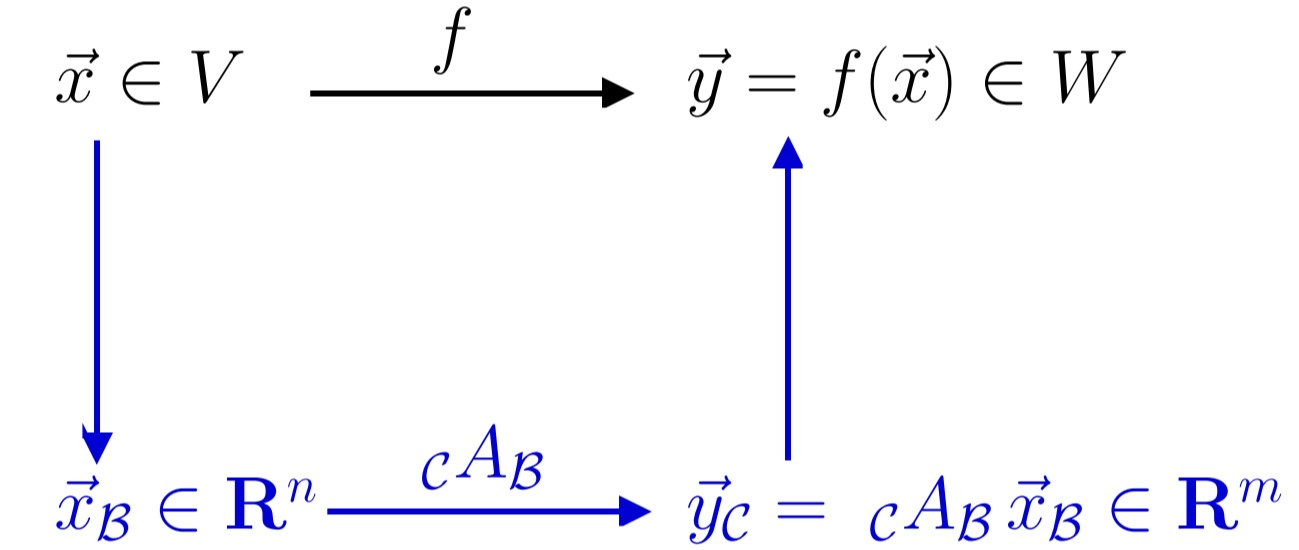
\includegraphics[scale=0.17]{abbildungsmatrix}
\end{center}

\ssect{Kern, Bild und Dimension}

Sei $f: V \rightarrow W$ eine lineare Abbildung von $V$ nach $W$.
Dann heisst die Menge $\ker(f) = \{ \vec{x} \in V \mid f(\vec{x}) = \vec{0} \in W \}$ der \textbf{Kern von $f$}.
Die Menge $\im(f) = \{ f(\vec{x}) \in W \mid \vec{x} \in V \}$ heisst das \textbf{Bild von $f$}.

\textbf{Satz:} Es gilt:
\begin{itemize}
    \item $\ker(f) = f^{-1}(\{ \vec{0} \})$, das Urbild von $\{ \vec{0} \}$.
    $\ker(f)$ ist ein Unterraum von $V$.
    \item $\im(f) = f(V)$, der Bildraum von $V$.
    $\im(f)$ ist ein Unterraum von $W$.
\end{itemize}

Es gilt:
\vspace{-0.8em}
\begin{align*}
    rg(A) &= \text{ \# der führenden Einsen in der Matrix $A$ auf ZSF} \\
    &= \text{ Maximale \# der l.u.\ Spaltenvektoren von $A$} \\
    &= \dim(\im(f))
\end{align*}
\vspace{-1.8em}

\textbf{Satz:} Seien $V$ und $W$ Vektorräume.
Sei $f: V \rightarrow W$ eine lineare Abbildung.
Dann ist:
\[\dim(V) = \dim(\ker(f)) + \dim(\im(f))\]

\sssect{Rezept zur Bestimmung von $\ker(f)$ und $\im(f)$}
\begin{enumerate}
    \item Wir bestimmen die Abbildungsmatrix $A$.
    \item Wir betrachten das homogene lineare LGS $A \vec{x} = \vec{0}$ und wenden das Gauss-Verfahren an.
    \item $\ker(f)$ und $\im(f)$ können wie folgt abgelesen werden:
    \begin{itemize}
        \item $\ker(f)$ ist die Lösungsmenge von $A \vec{x} = \vec{0}$ und $\dim(\ker(f)) = $ Anzahl der freien Variablen.
        \item $\dim(\im(f)) = $ Anzahl der führenden Variablen.
        Die führenden Einsen zeigen eine mögliche Auswahl von linear unabhängigen Spaltenvektoren der Abbildungsmatrix $A$.
        Diese Spaltenvektoren bilden eine Basis von $\im(f)$.
    \end{itemize}
\end{enumerate}

\ssect{Eigenschaften}

Es seien $f: V \rightarrow W$ und $g: V \rightarrow W$ lineare Abbildungen mit den Darstellungsmatrizen $A, B$.
Es gilt:
\begin{itemize}
    \item Die Abbildung $f + g$ ist linear und wird durch $A + B$ dargestellt.
    \item Für $k \in \R$ ist die Abbildung $k \ f$ linear und wird durch $k \ A$ dargestellt.
\end{itemize}

Es seien $f: V \rightarrow W$ und $g: W \rightarrow Z$ lineare Abbildungen mit den Darstellungsmatrizen $A \in \R^{r \times n}$ und $B \in \R^{m \times r}$.
Dann ist die Komposition $g \comp f$ linear und wird durch $BA$ dargestellt.

\textbf{Satz:} Sei $\dim(V) = \dim(W) = n$ und $f: V \rightarrow W$ eine lineare Abbildung mit der $n \times n$ Darstellungsmatrix $A$.
\begin{itemize}
    \item Die folgenden Äquivalenzen gelten:
    \begin{alignat*}{2}
        f \text{ ist bijektiv} &\Leftrightarrow \ker(f) = \{ \vec{0}_V \} &&\Leftrightarrow \im(f) = W \\ &\Leftrightarrow rg(A) = n &&\Leftrightarrow A \text{ ist invertierbar} \\
        &\Leftrightarrow \det(A) \neq 0
    \end{alignat*}
    \item Ist die lineare Abbildung $f$ bijektiv, dann ist die Umkehrabbildung $f^{-1}: W \rightarrow V$ linear und bijektiv.
    Die Darstellungsmatrix von $f^{-1}$ ist $A^{-1}$, die Inverse zu $A$.
\end{itemize}

\ssect{Basiswechsel}

Seien $\B = (\vec{b}_1, \dots, \vec{b}_n)$ und $\C = (\vec{c}_1, \dots, \vec{c}_n)$ zwei Basen des Vektorraumes $V$.
Dann nennt man die $n \times n$ Matrix ${_\C}T{_\B}$, deren Spaltenvektoren die Koordinatenvektoren der Basisvektoren $\vec{b}_k \in \B$ bzgl.\ Basis $\C$ sind, die \textbf{Basistransformationsmatrix $\B$ auf $\C$}.
Es gilt also:
\[{_\C}T{_\B} = \leftidx{_\C}{\left( (\vec{b}_1)_\C \ \dots \ (\vec{b}_n)_\C \right)}{_\B} \]
Man kann sich $\B$ als \emph{alte} Basis und $\C$ als \emph{neue} Basis vorstellen.
Dann sind die Spalten von ${_\C}T{_\B}$ die alten Basisvektoren im neuen Gewand.

\textbf{Satz:} Die Basistransformationsmatrix ${_\C}T{_\B}$ von $\B$ auf $\C$ ist eindeutig bestimmt und invertierbar mit $({_\C}T{_\B})^{-1} = {_\B}T{_\C}$

Die \textbf{Basistransformationsmatrix} ${_\C}T{_\B}$ ergibt sich mit dem Gauss-Jordan-Verfahren
für zwei beliebige Basen:
\[\left( \vec{c}_1 \ \vec{c}_2 \mid \vec{b}_1 \ \vec{b}_2 \right) \Leftrightarrow \left( I_2 \mid {_\C}T{_\B} \right)\]

Wenn die alte Basis die Standardbasis ist, dann ist die Basistransformationsmatrix gleich der Inverse der Matrix, die durch die Basisvektoren der neuen Basis gebildet wird:
\[{_\B}T{_\S} = \leftidx{_\B}{\left( \vec{b}_1 \ \vec{b}_2 \ \vec{b}_3 \right)}{_\S^{-1}}\]
Ist die neue Basis die Standardbasis, dann ist die Basistransformationsmatrix gleich der Matrix, die durch die Basisvektoren der alten Basis gebildet wird:
\[{_\S}T{_\B} = \leftidx{_\S}{\left( \vec{b}_1 \ \vec{b}_2 \ \vec{b}_3 \right)}{_\B}\]

\textbf{Satz:} Gegeben sei ein $n$-dimensionaler Vektorraum $V$ mit zwei Basen $\B$ und $\C$ sowie eine lineare Abbildung $f: V \rightarrow V$.
Dann besteht zwischen den Abbildungsmatrizen ${_\B}A{_\B}$ und ${_\C}A{_\C}$ folgender Zusammenhang:
\[{_\C}A{_\C} = {_\C}T{_\B} \cdot {_\B}A{_\B} \cdot {_\B}T{_\C} = {_\C}T{_\B} \cdot {_\B}A{_\B} \cdot {_\C}T{_\B^{-1}}\]

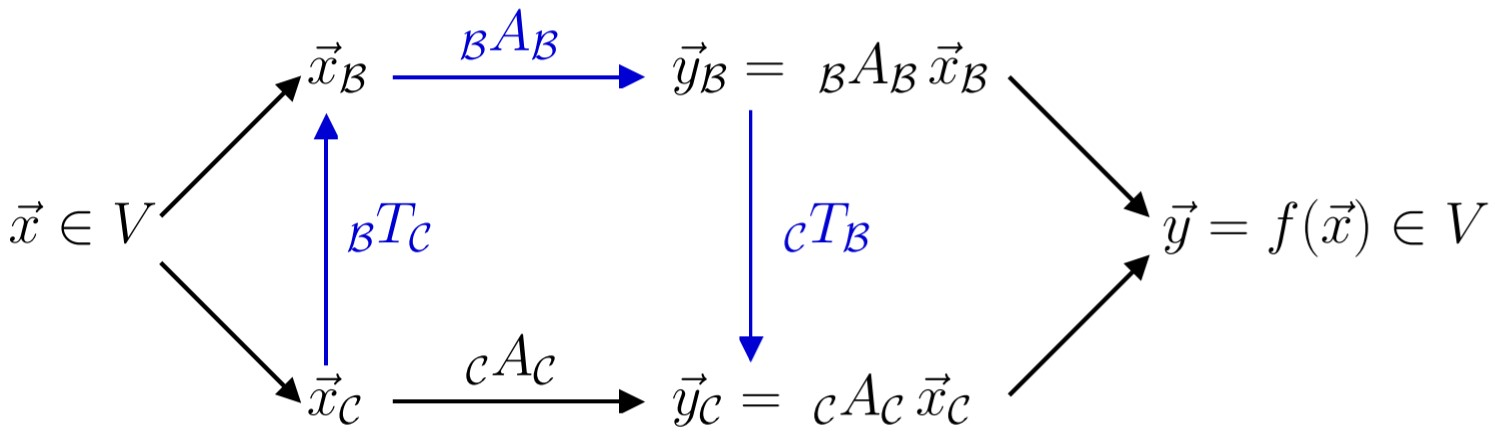
\includegraphics[scale=0.22]{basiswechsel}

\ssect{Geometrische Transformationen}

\sssect{Orthogonale Projektion}

\textbf{Orthogonalprojektion auf die $x$-Achse:}
\[\vec{x} \mapsto f(\vec{x}) = \left(
\begin{array}{cc}
    1 & 0 \\ 0 & 0
\end{array}
\right) \vec{x} = \left(
\begin{array}{c}
    x \\ 0
\end{array}
\right)\]

\textbf{Orthogonalprojektion auf die $y$-Achse:}
\[\vec{x} \mapsto f(\vec{x}) = \left(
\begin{array}{cc}
    0 & 0 \\ 0 & 1
\end{array}
\right) \vec{x} = \left(
\begin{array}{c}
    0 \\ y
\end{array}
\right)\]

\hrulefill

\begin{multicols}{2}
    \begin{itemize}
        \item Gerade $g: ax + by = 0$
        \item Mit $a^2 + b^2 = 1$
    \end{itemize}
    \[\left(
    \begin{array}{cc}
        1-a^2 & -ab \\ -ab & 1-b^2
    \end{array}
    \right)\]
\end{multicols}

\hrulefill

\begin{multicols}{2}
    \raggedright
    \begin{itemize}
        \item Gerade $g: 2x - y = 0$\\
        \item Normiert $g: \frac{2}{\sqrt{5}} x - \frac{1}{\sqrt{5}} y = 0$
    \end{itemize}
    \[\frac{1}{5} \cdot \left(
    \begin{array}{cc}
        1 & 2 \\ 2 & 4
    \end{array}
    \right)\]
\end{multicols}

\hrulefill

\textbf{Orthogonale Projektion auf die Ebene:}
\begin{itemize}
    \item $E: ax + by + cz = 0$
    \item $a^2 + b^2 + c^2 = 1$
\end{itemize}
\[P = \left(
\begin{array}{ccc}
    1-a^2 & -ab   & -ac   \\
    -ab   & 1-b^2 & -bc   \\
    -ac   & -bc   & 1-c^2
\end{array}
\right)\]
$P = E - \vec{n} \cdot \vec{n}^T$

\sssect{Spiegelung}

\textbf{Spiegelung an der $y$-Achse:}
\[\vec{x} \mapsto f_{S_y}(\vec{x}) = \left(
\begin{array}{cc}
    -1 & 0 \\ 0 & 1
\end{array}
\right) \vec{x} = \left(
\begin{array}{c}
    -x \\ y
\end{array}
\right)\]

\textbf{Spiegelung an der $x$-Achse:}
\[\vec{x} \mapsto f_{S_x}(\vec{x}) = \left(
\begin{array}{cc}
    1 & 0 \\ 0 & -1
\end{array}
\right) \vec{x} = \left(
\begin{array}{c}
    x \\ -y
\end{array}
\right)\]

\textbf{Spiegelung am Nullpunkt:}
\[\vec{x} \mapsto f_{S_N}(\vec{x}) = \left(
\begin{array}{cc}
    -1 & 0 \\ 0 & -1
\end{array}
\right) \vec{x} = \left(
\begin{array}{c}
    -x \\ -y
\end{array}
\right)\]

\hrulefill

\begin{multicols}{2}
    \begin{itemize}
        \item Gerade $g: ax + by = 0$
        \item Mit $a^2 + b^2 = 1$
    \end{itemize}
    \[\left(
    \begin{array}{cc}
        1 - 2a^2 & -2ab \\ -2ab & 1 - 2b^2
    \end{array}
    \right)\]
\end{multicols}

\hrulefill

\begin{multicols}{2}
    \raggedright
    \begin{itemize}
        \item Gerade $g: x + 7y = 0$
        \item Normiert $g: \frac{1}{\sqrt{50}}x + \frac{7}{\sqrt{50}}y = 0$
    \end{itemize}
    \[\frac{1}{50} \cdot \left(
    \begin{array}{cc}
        48 & -14 \\ -14 & -48
    \end{array}
    \right)\]
\end{multicols}

\hrulefill

\textbf{Spiegelung an der Ebene:}
\begin{itemize}
    \item $E: ax + by + cz = 0$
    \item $a^2 + b^2 + c^2 = 1$
\end{itemize}
\[S = \left(
\begin{array}{ccc}
    1-2a^2 & -2ab   & -2ac   \\
    -2ab   & 1-2b^2 & -2bc   \\
    -2ac   & -2bc   & 1-2c^2
\end{array}
\right)\]
$S = E - 2 \vec{n} \cdot \vec{n}^T$

\sssect{Streckung}

\textbf{Streckung längst der $x$-Achse um den Faktor $k$:}
\[\vec{x} \mapsto f_x(\vec{x}) = \left(
\begin{array}{cc}
    k & 0 \\
    0 & 1
\end{array}
\right) \vec{x} = \left(
\begin{array}{c}
    kx \\ y
\end{array}
\right)\]

\textbf{Streckung längst der $y$-Achse um den Faktor $k$:}
\[\vec{x} \mapsto f_y(\vec{x}) = \left(
\begin{array}{cc}
    1 & 0 \\
    0 & k
\end{array}
\right) \vec{x} \left(
\begin{array}{c}
    x \\ ky
\end{array}
\right)\]

\textbf{Zentrische Streckung vom Nullpunkt aus mit Faktor $k$:}
\[\vec{x} \mapsto f_{zs}(\vec{x}) = \left(
\begin{array}{cc}
    k & 0 \\
    0 & k
\end{array}
\right) \vec{x} = \left(
\begin{array}{c}
    kx \\ ky
\end{array}
\right)\]

\begin{center}
    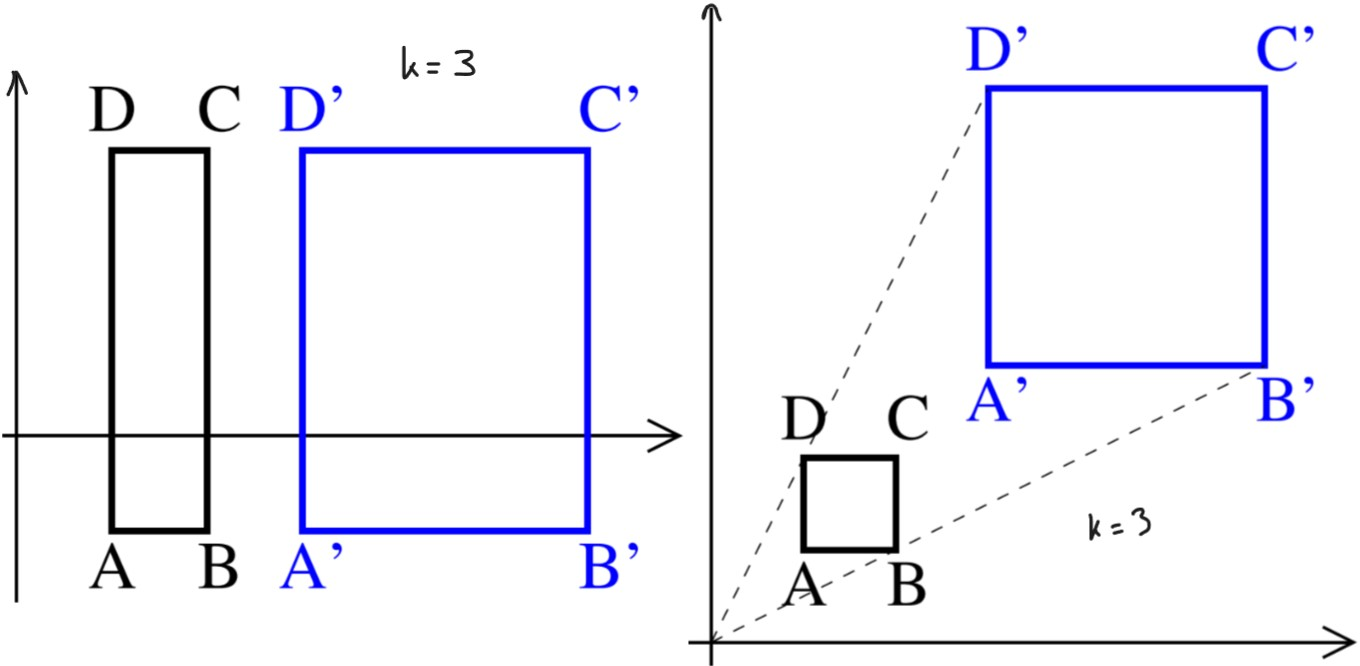
\includegraphics[scale=0.17]{streckung}
\end{center}

Faktor $\lambda$: $\left(
\begin{array}{ccc}
    \lambda & 0       & 0       \\
    0       & \lambda & 0       \\
    0       & 0       & \lambda
\end{array}
\right)$

\sssect{Scherung}

\textbf{Scherung längst der $x$-Achse mit Faktor $k$:}
\[\vec{x} \mapsto f(\vec{x}) = \left(
\begin{array}{cc}
    1 & k \\ 0 & 1
\end{array}
\right) \left(
\begin{array}{c}
    x \\ y
\end{array}
\right) = \left(
\begin{array}{c}
    x + ky \\ y
\end{array}
\right)\]

\textbf{Scherung längst der $y$-Achse mit Faktor $y$:}
\[\vec{x} \mapsto f(\vec{x}) = \left(
\begin{array}{cc}
    1 & 0 \\ k & 1
\end{array}
\right) \left(
\begin{array}{c}
    x \\ y
\end{array}
\right) = \left(
\begin{array}{c}
    x \\ kx + y
\end{array}
\right)\]

\sssect{Drehung}

\begin{multicols}{2}
    \begin{itemize}
        \item Um den Ursprung
        \item Um den Winkel $\varphi$
    \end{itemize}
    \[\left(
    \begin{array}{cc}
        \cos(\varphi) & -\sin(\varphi) \\
        \sin(\varphi) & \cos(\varphi)
    \end{array}
    \right)\]
\end{multicols}

\textbf{Drehung um den Winkel $\varphi$}

$x$-Achse: $\left(
\begin{array}{ccc}
    1 & 0             & 0              \\
    0 & \cos(\varphi) & -\sin(\varphi) \\
    0 & \sin(\varphi) & \cos(\varphi)
\end{array}
\right)$

$y$-Achse: $\left(
\begin{array}{ccc}
    \cos(\varphi)  & 0 & \sin(\varphi) \\
    0              & 1 & 0             \\
    -\sin(\varphi) & 0 & \cos(\varphi)
\end{array}
\right)$

$z$-Achse: $\left(
\begin{array}{ccc}
    \cos(\varphi) & -\sin(\varphi) & 0 \\
    \sin(\varphi) & \cos(\varphi)  & 0 \\
    0             & 0              & 1
\end{array}
\right)$

        \newpage

        \sect{Prüfungsaufgaben}

\ssect{FS2022}

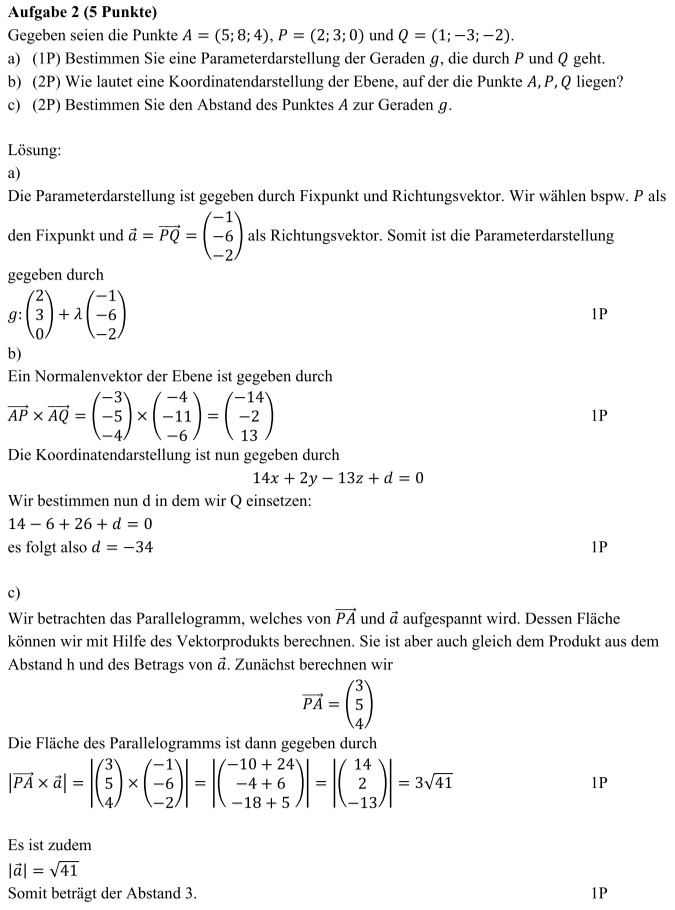
\includegraphics[scale=0.45]{fs2022-aufgabe-2}

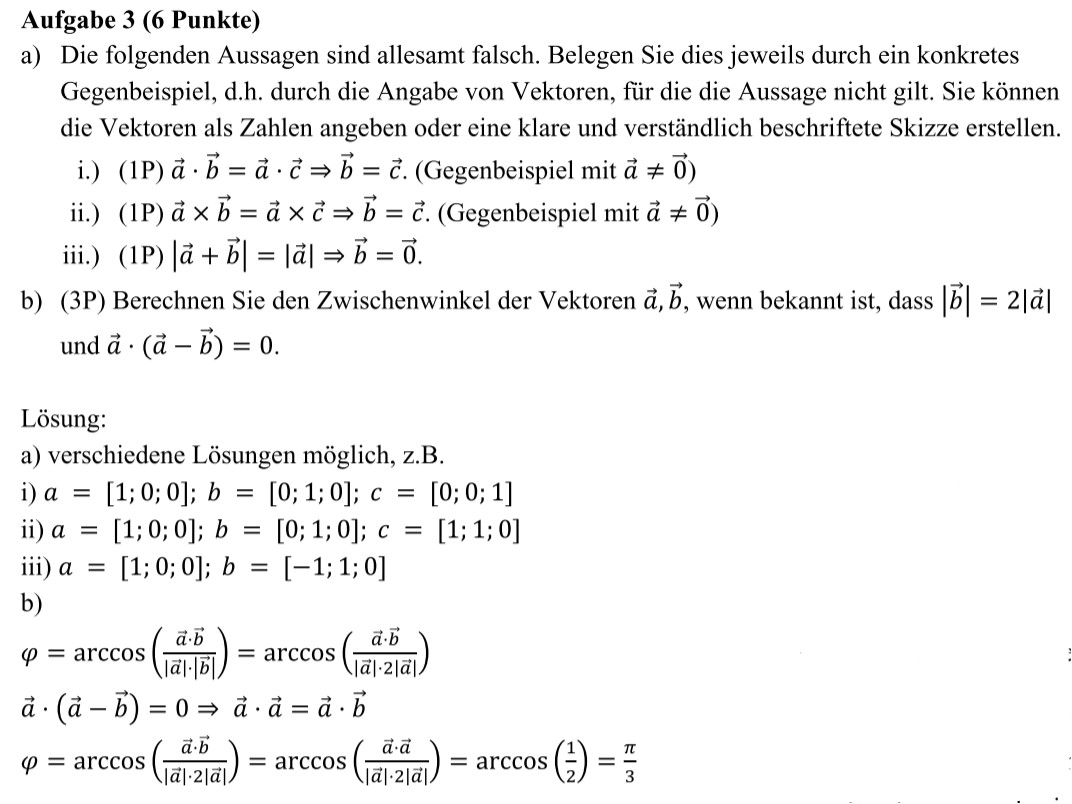
\includegraphics[scale=0.28]{fs2022-aufgabe-3}

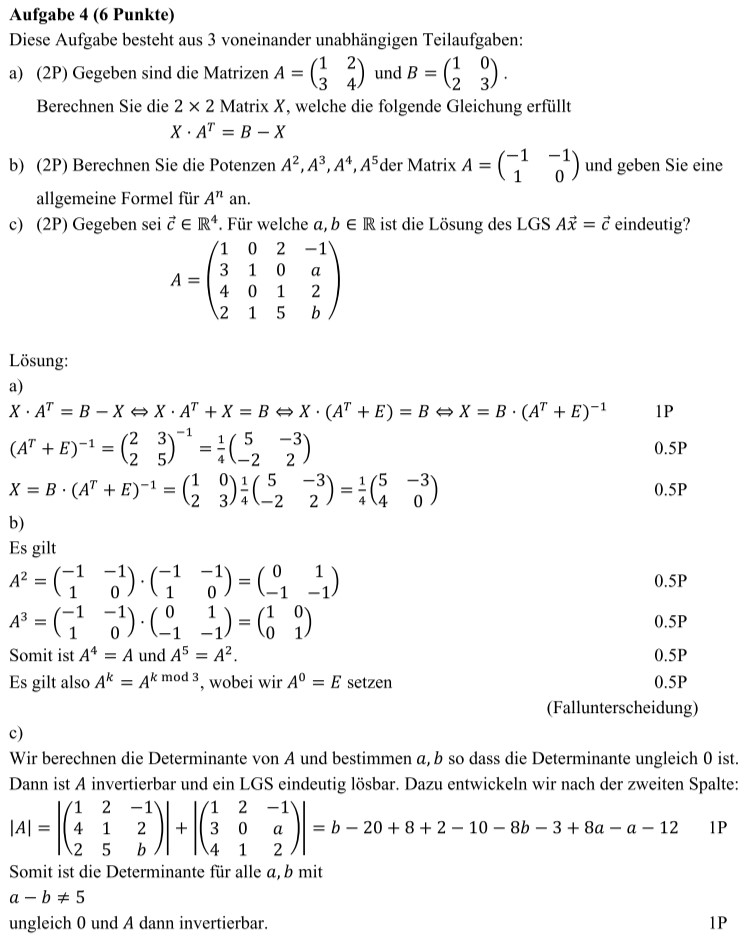
\includegraphics[scale=0.45]{fs2022-aufgabe-4}

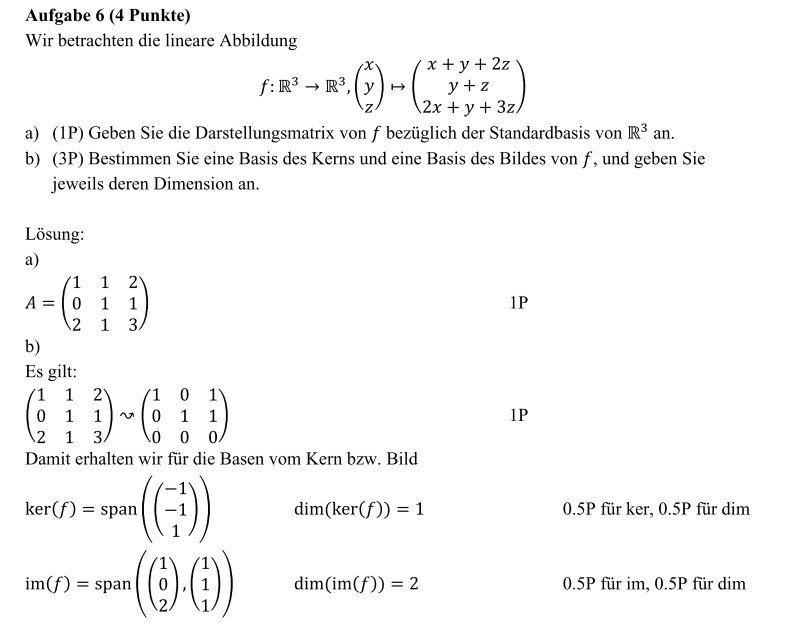
\includegraphics[scale=0.43]{fs2022-aufgabe-6}

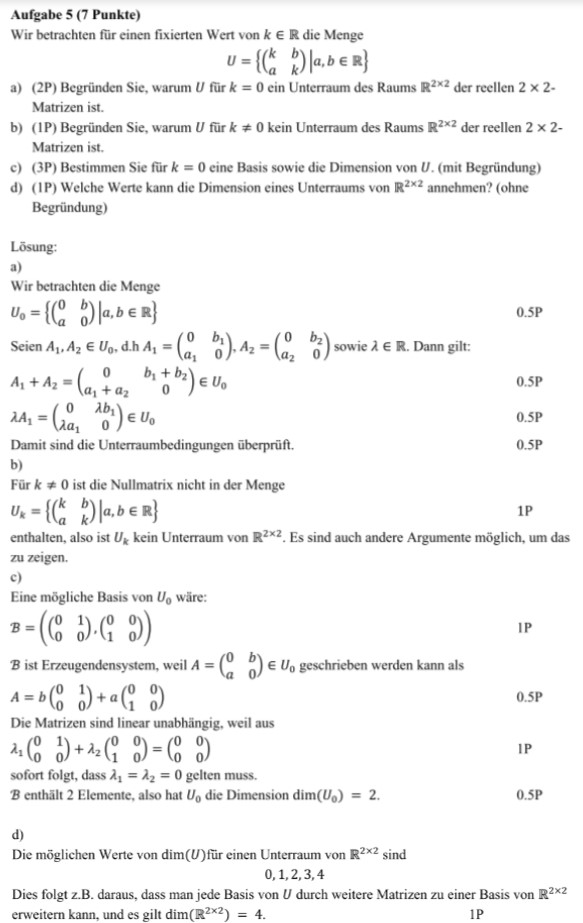
\includegraphics[scale=0.47]{fs2022-aufgabe-5}

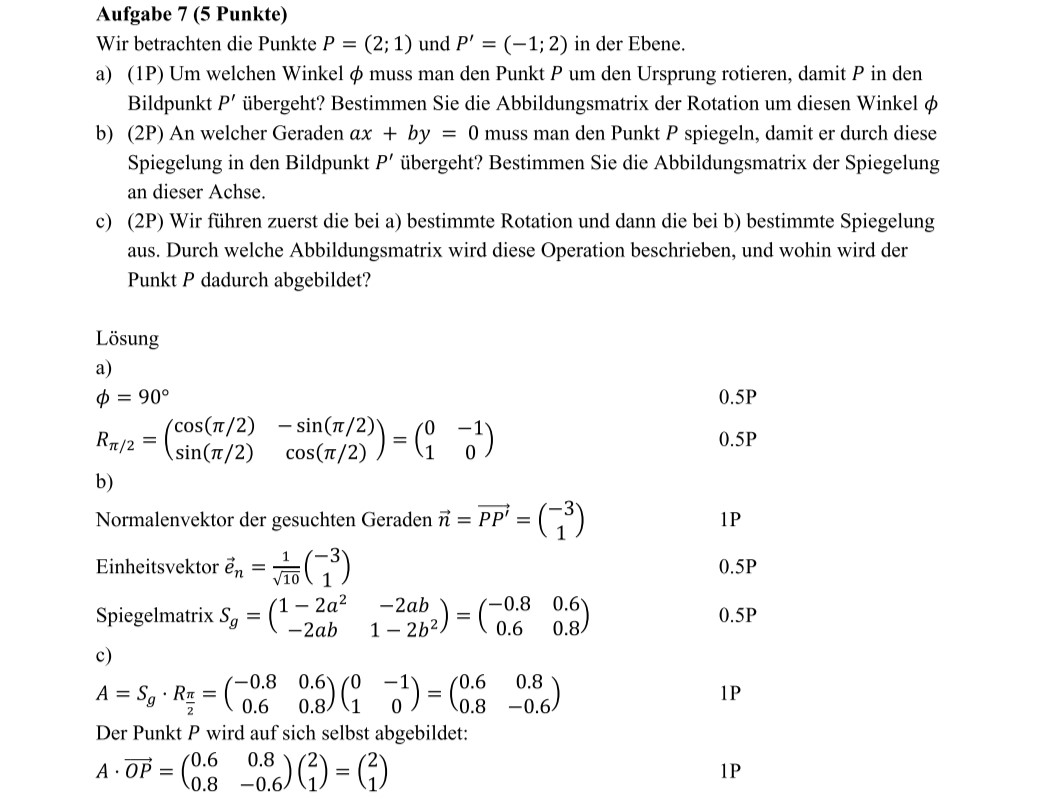
\includegraphics[scale=0.321]{fs2022-aufgabe-7}

\ssect{FS2021}

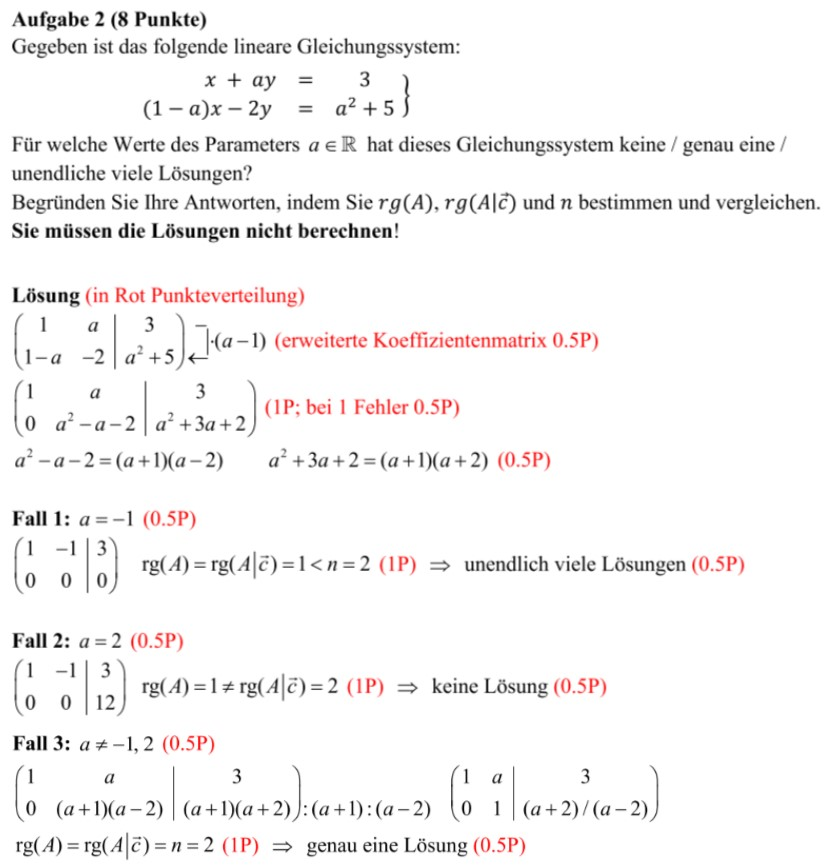
\includegraphics[scale=0.3925]{fs2021-aufgabe-2}

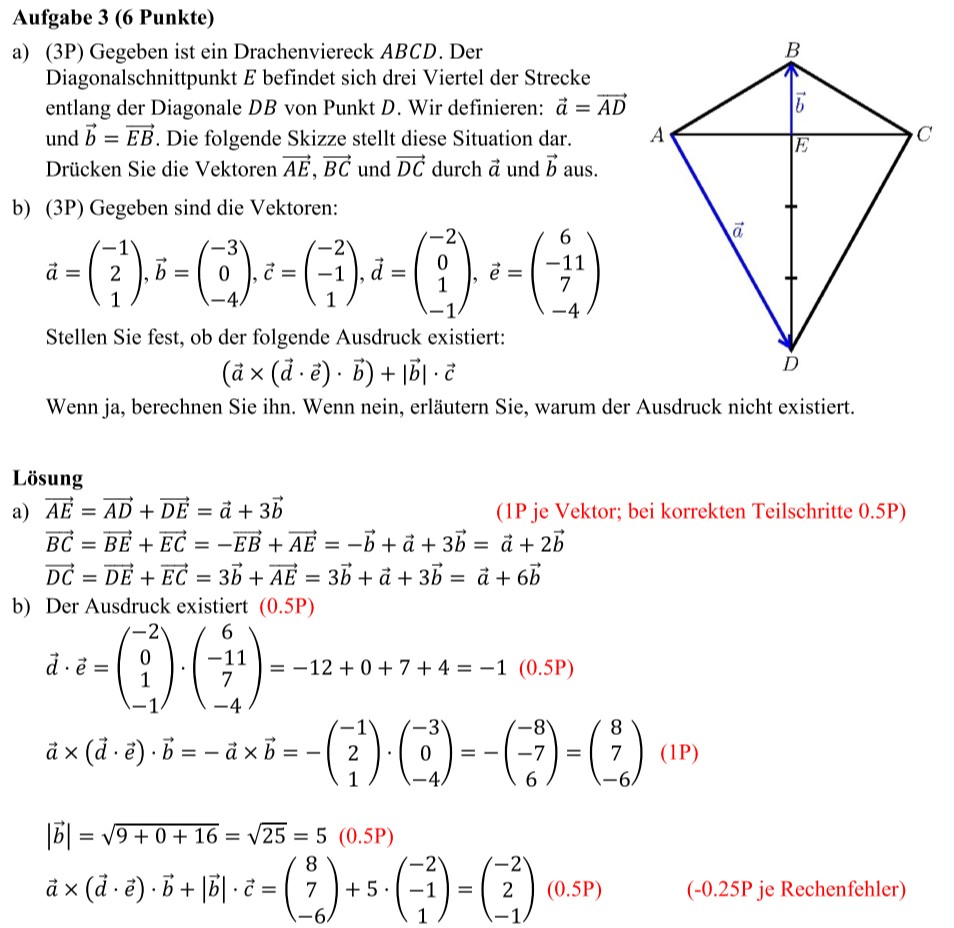
\includegraphics[scale=0.35]{fs2021-aufgabe-3}

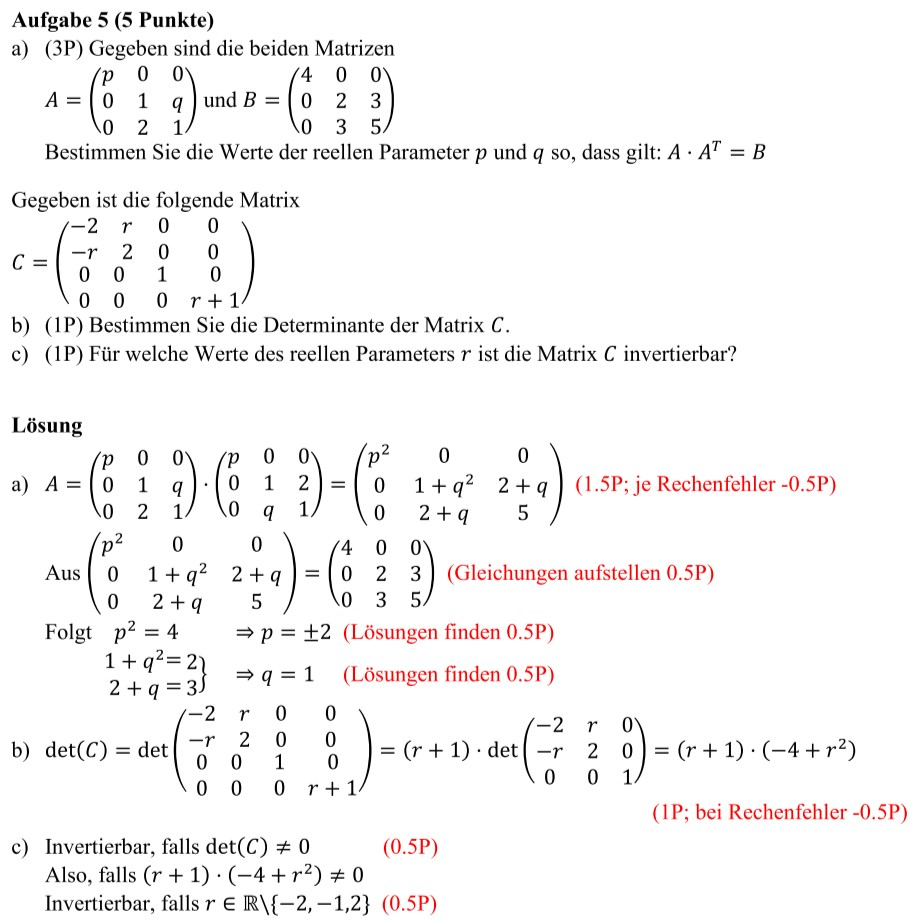
\includegraphics[scale=0.3]{fs2021-aufgabe-5}

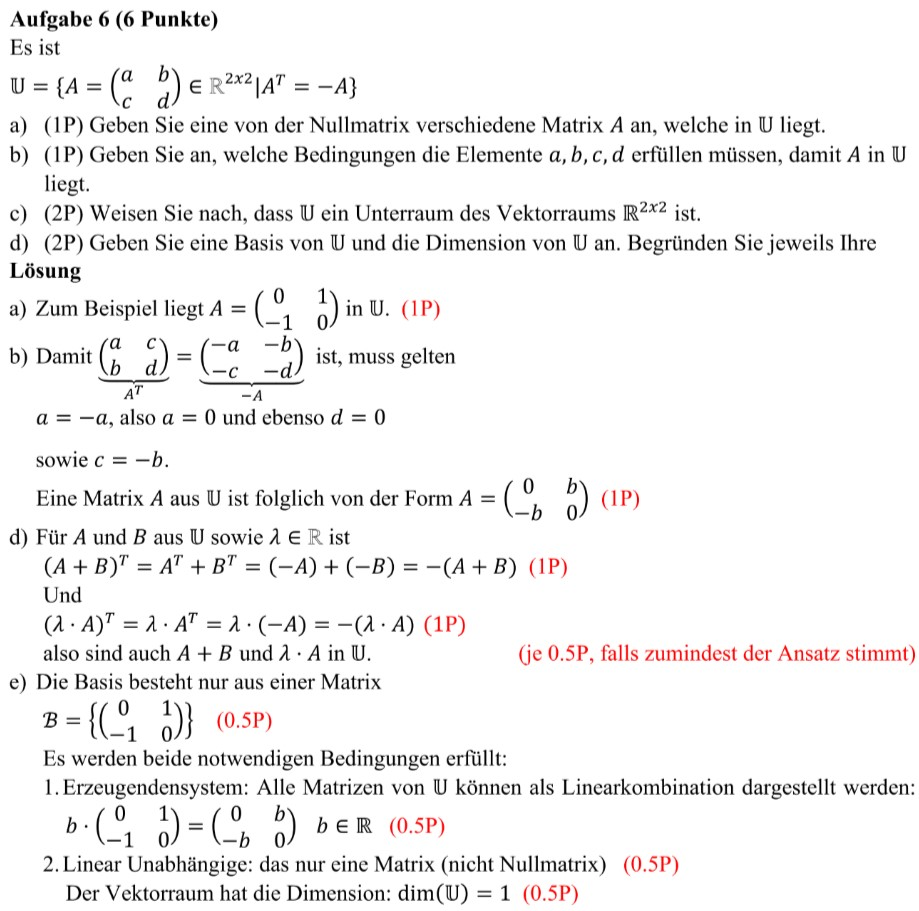
\includegraphics[scale=0.37]{fs2021-aufgabe-6}

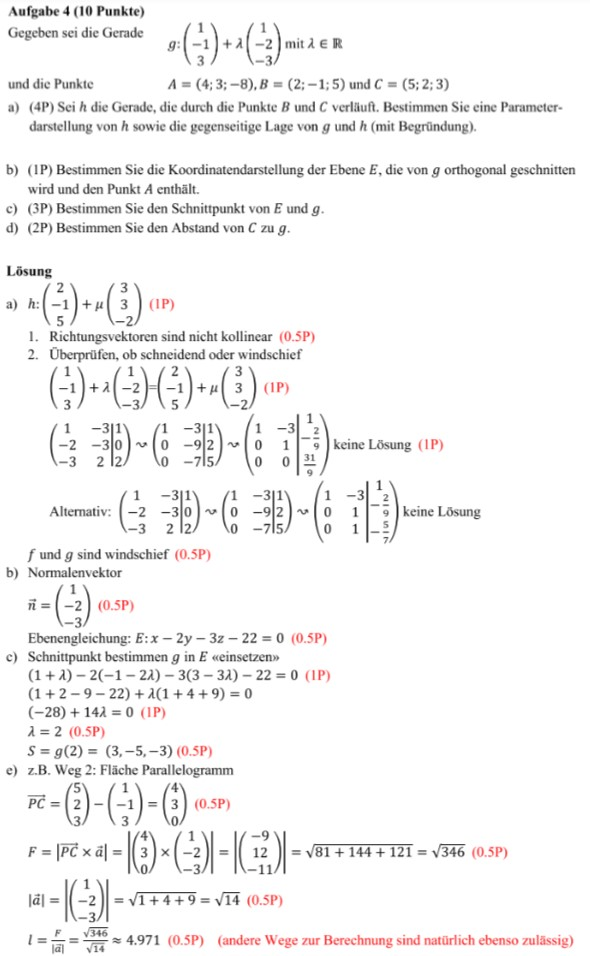
\includegraphics[scale=0.6]{fs2021-aufgabe-4}
    \end{multicols*}
\end{document}